\documentclass[a4paper]{report}
\usepackage[fontsize=12pt]{scrextend}
\usepackage[utf8]{inputenc}
\usepackage{adjustbox}
\usepackage{amsmath}
\usepackage{hyperref}
\usepackage{hyperxmp}
\usepackage{textcomp}
\usepackage[most]{tcolorbox}
\tcbuselibrary{minted}
\usemintedstyle{tango}
\usepackage{xcolor}
\usepackage[
    type={CC},
    modifier={zero},
    version={1.0},
]{doclicense}
\usepackage{fontawesome5}
\definecolor{hcode}{RGB}{240, 240, 224}
\usepackage{shadowtext}
\usepackage{luacolor}
\usepackage{lua-ul}
\usepackage{listings}
\usepackage{enumitem}
\usepackage{svg}
\usepackage{multirow}
\usepackage{booktabs}
\usepackage{svg}
\usepackage{listings}
%\usepackage{algorithm}
\usepackage{pgfplots}
\definecolor{mygreen}{RGB}{28,172,0} % color values Red, Green, Blue
\definecolor{mylilas}{RGB}{170,55,241}
\usetikzlibrary{matrix}
\setcounter{tocdepth}{3}
\setcounter{secnumdepth}{3}
\def\codefont{
  \fontspec{Courier New}
  \fontsize{9pt}{11pt}\selectfont}
\definecolor{codebgcolor}{HTML}{EDEDED}
% Define a custom environment for dedication
\newenvironment{dedication}
{
    \cleardoublepage
    \thispagestyle{empty}
    \vspace*{7cm}
    \begin{center}
    \bfseries \normalsize Dedication \par
    \end{center}
    \itshape
}
{
    \cleardoublepage
}
\newenvironment{code}
{\begin{center}
    \begin{tikzpicture}
      \node [fill=codebgcolor,rounded corners=5pt]
      \bgroup
      \bgroup\codefont
      \begin{tabular}{l}}
      {\end{tabular}
      \egroup
      \egroup;
    \end{tikzpicture}
  \end{center}}

\newcommand\numRowsK{3}
\newcommand\numColsK{3}
\newcommand{\K}[2]{% #1: row, #2: col
    \edef\Kcol##1##2##3{###2}%
    \edef\Krow##1##2##3{\noexpand\Kcol###1}%
    \Krow
        {1 0 1}
        {0 1 0}
        {1 0 1}%
}

\usepackage{listofitems} % for \readlist to create arrays
\usetikzlibrary{arrows.meta} % for arrow size
\usepackage[outline]{contour} % glow around text
\contourlength{1.4pt}

% COLORS
\usepackage{xcolor}
\colorlet{myred}{red!80!black}
\colorlet{myblue}{blue!80!black}
\colorlet{mygreen}{green!60!black}
\colorlet{myorange}{orange!70!red!60!black}
\colorlet{mydarkred}{red!30!black}
\colorlet{mydarkblue}{blue!40!black}
\colorlet{mydarkgreen}{green!30!black}

% STYLES
\tikzset{
  >=latex, % for default LaTeX arrow head
  node/.style={thick,circle,draw=myblue,minimum size=22,inner sep=0.5,outer sep=0.6},
  node in/.style={node,green!20!black,draw=mygreen!30!black,fill=mygreen!25},
  node hidden/.style={node,blue!20!black,draw=myblue!30!black,fill=myblue!20},
  node convol/.style={node,orange!20!black,draw=myorange!30!black,fill=myorange!20},
  node out/.style={node,red!20!black,draw=myred!30!black,fill=myred!20},
  connect/.style={thick,mydarkblue}, %,line cap=round
  connect arrow/.style={-{Latex[length=4,width=3.5]},thick,mydarkblue,shorten <=0.5,shorten >=1},
  node 1/.style={node in}, % node styles, numbered for easy mapping with \nstyle
  node 2/.style={node hidden},
  node 3/.style={node out}
}
\def\nstyle{int(\lay<\Nnodlen?min(2,\lay):3)} % map layer number onto 1, 2, or 3
\pgfplotsset{compat=1.16}
\usepackage{float}
\usepackage{tikz}
\usepackage{amssymb}
\usepackage{xpatch}
\newlength{\chaptertopskip}
\setlength{\chaptertopskip}{10pt}
\makeatletter
\xpatchcmd{\@makechapterhead}{\vspace*{50\p@}}{\vspace*{\chaptertopskip}}{\typeout{Success}}{\typeout{Failure!!!}}
\makeatother
\usepackage{caption}
\usepackage{fontspec}
\usepackage[toc]{appendix}
\usepackage{verbatim}
\usepackage{xcolor,graphicx}
\usepackage[top=0.6in,bottom=0.6in,right=1in,left=1in]{geometry}
\graphicspath{{images/}{images_pfe/}}
\newlength\figureheight
\newlength\figurewidth
\usepackage{tocloft}
\usepackage[chapter]{algorithm}
\usepackage{algpseudocode}
\usepackage{polyglossia}
\setmainlanguage{english}
\setotherlanguage{arabic}
\newfontfamily\arabicfont[Script=Arabic,Scale=1.1]{Scheherazade}
\setlength{\fboxrule}{2pt}
\setlength{\fboxsep}{0pt}
\thispagestyle{empty}
\addto\captionsenglish{
  \renewcommand{\contentsname}%
    {Table of Contents}%
}

\usepackage{etoolbox}
\usepackage{fancyhdr}
\pagestyle{fancy}
\fancyhf{}
\fancyhead[EL]{\nouppercase\leftmark}
\fancyhead[OR]{\nouppercase\rightmark}
\fancyhead[ER,OL]{\thepage}

\makeatletter
\AtBeginDocument{%
  \let\l@algorithm\l@figure%
  \let\listofalgorithms\listoffigures
  \let\@cftmakeloatitle\@cftmakeloftitle
  \patchcmd{\listofalgorithms}{\@cftmakeloftitle}{\@cftmakeloatitle}{}{}%
  \patchcmd{\listofalgorithms}{\@starttoc{lof}}{\@starttoc{loa}}{}{}%
  \patchcmd{\@cftmakeloatitle}{\listfigurename}{\listalgorithmname}{}{}%
 
  \patchcmd{\@chapter}{\addtocontents}{%
    \addtocontents{loa}{\protect\addvspace{10\p@}}%
    \addtocontents}{}{}%
}
\makeatother
\usepackage{afterpage}
\newcommand\blankpage{%
    \null
    \thispagestyle{empty}%
    \addtocounter{page}{-1}%
    \newpage}

\renewcommand{\cfttoctitlefont}{\hfill\Huge}
\renewcommand{\cftaftertoctitle}{\vspace{0.8ex}\endgraf\rule{\linewidth}{0.5pt}}
\renewcommand{\cftloftitlefont}{\hfill\Huge}
\renewcommand{\cftafterloftitle}{\vspace{0.8ex}\endgraf\rule{\linewidth}{0.5pt}}

\begin{document}
\renewcommand{\refname}{Webliography}
\renewcommand{\bibname}{Webliography}
\begin{titlepage}
    \centering
    {\textsc{{\small République Algérienne Démocratique et Populaire}}}\\
    \begin{Arabic}
    {\large الجمهورية الجزائرية الديمقراطية الشعبية}\\
	\end{Arabic}
    {\textsc{\small Ministère de L'Enseignement Supérieur et de la Recherche Scientifique}}\\
        \begin{Arabic}
        \large {وزارة التعليم العالي و البحث العلمي} \\
	\end{Arabic}
\rule{\linewidth}{0.3mm} \\[0.4cm]
\textbf{\small {INSTITUTE OF ELECTRICAL AND \\ELECTRONIC ENGINEERING}}\\
\begin{Arabic}
    \normalsize{معهد الهندسة الكهربائية و الالكترونيك}
\end{Arabic}\\
\begin{minipage}{5cm}
	\begin{center}
		\includegraphics[width=5cm]{umbb2.png}
	\end{center}
\end{minipage}
\\\textbf{University of Boumerdes}\\
\vspace{10mm}
{\large \bfseries Final Year Project Report}\\[0.5cm]
{\large in Partial Fulfillment of the Requirements
of the Degree of:\\
\textbf{‘LICENCE’}}\\[0.5cm]
{\large Submitted to:\\ \vspace{0.5cm}
\bfseries{Department of Electronics}}\\
\vspace{5mm}
{\large Titled:\\
{\Large \bfseries\fbox{\parbox[t][3.5em][c]{\textwidth}{\centering End-to-End Voice Command Security System Using Deep Learning Algorithms}}}\\

\vspace{15mm}


\noindent
\begin{minipage}{0.5\textwidth}
    \vspace{-7mm}
  \begin{flushleft} \large
    \emph{Presented By :}\\\vspace{0.5cm}
    - \textsc{Albourm} Amar \\
    - \textsc{Hadj Idris} Nassim \\
    - \textsc{Naga} Abderrahemene \\
  \end{flushleft}
\end{minipage}
\begin{minipage}{0.4\textwidth}
\vspace{-20mm}
  \begin{flushright} \large
    \begin{flushleft} \large
    \emph{Supervised By :} \\\vspace{0.5cm}
    - Dr. \textsc{Tabet} Youcef\\[0.1cm]
    \end{flushleft}

  \end{flushright}
\end{minipage}\\[1cm]
\vspace{16mm}

{\large Promotion : 2023/2024}
\rule{\linewidth}{0.3mm} \\[0.4cm]
{\small \textsc{\textbf{IGEE} \color{blue} \textbf{2024}$\color{blue} ^©$}}}
\end{titlepage}
\pagenumbering{roman}
\begin{abstract}

\addcontentsline{toc}{chapter}{Abstract}
Current security systems have trouble adjusting to new threats, dealing with complexity, and getting useful information from data. These problems make it hard for them to react quickly in dangerous situations. But this project suggests a new way. It uses machine learning and embedded systems to make a system that can adapt. Convolutional neural networks are trained to recognize specific commands, enabling voice-based interaction with critical machinery or electronic devices. This hands-free solution improves safety and efficiency during emergencies, particularly beneficial in industrial settings.
\end{abstract}
\afterpage{\blankpage}
\begin{dedication}
\addcontentsline{toc}{chapter}{Dedication}
\setcounter{page}{2} 
\noindent
\textit{We dedicate this memoir to our families, whose unwavering support and encouragement have been our foundation. Thank you..\\\\
To our supervisor, Dr.Tabet Youcef, thank you for your invaluable guidance and belief in our vision..\\\\
With heartfelt gratitude,}
\noindent
\end{dedication}

\clearpage
\tableofcontents
\newpage
\listoffigures
\newpage
\listofalgorithms

\chapter*{General Introduction}
\pagenumbering{arabic}
\addcontentsline{toc}{chapter}{General Introduction}
In this rapid era of technological development, the integration of artificial intelligence
into everyday applications has become increasingly commonplace. Among these applications
Speech recognition systems have drawn tremendous attention. These systems allow hands-free control of
devices, thus assuring ease as well as safety, particularly in industrial scenes.

This project addresses developing a robust speech recognition system using state-of-the-art machine learning techniques. Utilizing convolutional neural networks (CNNs) and long short-term memory (LSTM) networks, the system is designed to recognize specific voice commands. 

The developed system will be integrated onto a microcontroller, specifically the ESP32. This integration onto a microcontroller like the ESP32 is crucial for enabling the deployment of the speech recognition system in real-world scenarios, particularly in environments where edge computing capabilities are necessary.

The speech recognition system can operate efficiently and autonomously, offering hands-free control of devices in industrial settings and beyond.

The following sections of this report will delve into the theoretical foundations, methodological approaches, and practical implementations of the developed system. Through detailed analysis and discussion, this report aims to contribute insights into the development of efficient and adaptive speech recognition systems deployable on edge devices.
\vspace*{-3cm}
\chapter{Theoretical Framework}
\section{Artificial Neural Networks}
\normalsize{
In general, artificial neural networks \textbf{(ANNs)} are composed of artificial neurons. Each artificial neuron has a formal representation with $n$ inputs denoted as a vector $\vec{x}\in\mathbb{R}^n$. These inputs mimic the function of dendrites in biological neurons.
\begin{center}
\includegraphics[width=0.4\linewidth]{image.png}
\captionof{figure}{Model for a biological neuron}
\end{center}
The output of an artificial neuron corresponds to the axon of a biological neuron. Each input (indexed $1\leq i\leq n$) is associated with a weight (${w_1, w_2,...,w_n}$). Inputs undergo a combination process and pass through an activation function to generate an output. The network links neurons' outputs to inputs, forming an oriented graph, with vertices representing neurons and directed edges representing connections
\begin{figure}[H]
\begin{center}
\begin{tikzpicture}[>=latex]
\path
(0,0)     node[circle,draw,scale=2,inner sep=2pt] (S) {$\Sigma$}
+(90:2.5) node[circle,draw,inner sep=2.5pt] (b) {}
          node[above=1mm] {$b_1^{(2)}$}
+(-3.5,1.5)  node[circle,fill=green!50]  (x1) {$x_1$}
+(-3.5,0)    node[circle,fill=green!50]  (x2) {$x_2$}
+(-3.5,-1.5) node[circle,fill=green!50]  (x3) {$x_3$}
(2,0)    node[draw] (g) {$g$} node[above=3mm]{Activation}
+(15:3)  node[circle,fill=red!50]  (y1) {$\hat{y}_1$}
+(-15:3) node[circle,fill=red!50]  (y2) {$\hat{y}_2$};
\draw[->] (S)--(g);
\draw[->] (b)--(S);
\draw[->] (g)--(y1) node[pos=.6,above]{$\omega_{1,1}^{(3)}$};
\draw[->] (g)--(y2) node[pos=.6,below]{$\omega_{2,1}^{(3)}$};
\draw[->] (x1)--(S) node[pos=.4,above]{$\omega_{1,1}^{(2)}$};
\draw[->] (x2)--(S) node[pos=.4,above]{$\omega_{1,2}^{(2)}$};
\draw[->] (x3)--(S) node[pos=.4,above]{$\omega_{1,3}^{(2)}$};
\draw[blue] (1,0) circle(2.2);
\end{tikzpicture}
\end{center}
\caption{Model for artificial neuron}
\end{figure}
A group of input neurons comprises those neurons at the initial points of any complete path in the graph. Each input neuron has precisely one input, collectively representing an instance of the problem addressed by the \textbf{ANN}. Similarly, a collection of output neurons includes those neurons at the terminal points of any complete path in the graph. Each output neuron has precisely one output, and together they represent potential solutions to the problem tackled by the \textbf{ANN}.

Hidden neurons constitute those neurons that are neither input nor output neurons. Their quantity and arrangement into layers may differ, even for the same problem, but play a pivotal role in the network's performance.
\begin{figure}[H]
\begin{center}
    \begin{tikzpicture}[x=2.2cm,y=1.4cm]
  \message{^^JNeural network without arrows}
  \readlist\Nnod{4,5,5,5,3} % array of number of nodes per layer
  
  \message{^^J  Layer}
  \foreachitem \N \in \Nnod{ % loop over layers
    \def\lay{\Ncnt} % alias of index of current layer
    \pgfmathsetmacro\prev{int(\Ncnt-1)} % number of previous layer
    \message{\lay,}
    \foreach \i [evaluate={\y=\N/2-\i; \x=\lay; \n=\nstyle;}] in {1,...,\N}{ % loop over nodes
      
      % NODES
      \node[node \n] (N\lay-\i) at (\x,\y) {$a_\i^{(\prev)}$};
      
      % CONNECTIONS
      \ifnum\lay>1 % connect to previous layer
        \foreach \j in {1,...,\Nnod[\prev]}{ % loop over nodes in previous layer
          \draw[connect,white,line width=1.2] (N\prev-\j) -- (N\lay-\i);
          \draw[connect] (N\prev-\j) -- (N\lay-\i);
          %\draw[connect] (N\prev-\j.0) -- (N\lay-\i.180); % connect to left
        }
      \fi % else: nothing to connect first layer
      
    }
  }
  
  % LABELS
  \node[above=5,align=center,mygreen!60!black] at (N1-1.90) {input\\[-0.2em]layer};
  \node[above=2,align=center,myblue!60!black] at (N3-1.90) {hidden layer};
  \node[above=8,align=center,myred!60!black] at (N\Nnodlen-1.90) {output\\[-0.2em]layer};
  
\end{tikzpicture}
\end{center}
\caption{Layers of ANN}
\end{figure}
\textbf{\underline{Definition:}} Formally, a neural network is a hextuple (6-tuple) $\Gamma=(\mathcal{N}, \mathcal{E}, \mathbb{X}, \mathbb{Y}, \omega, \beta)$ where:\\
$\bullet$ $\mathcal{N}$ is a finite non-empty set of neurons\\
$\bullet$ $\mathcal{E} \subseteq \mathcal{N}^2$ is a non-empty set of oriented edges between neurons\\
$\bullet$ $\mathbb{X}\subset \mathcal{N}$ is a non-empty set of neurons in the input layer\\
$\bullet$ $\mathbb{Y}\subset \mathcal{N}$ is a non-empty set of neurons in the output layer\\
$\bullet$ $\omega\::\:\mathcal{E}\rightarrow\mathbb{R}$ is a weighting function\\
$\bullet$ $\beta\::\:\mathcal{N}\rightarrow\mathbb{R}$ is a function for network bias

\vspace{1cm}
Let us consider neuron \( j \) with its input \(\vec{x}_j = (x_{1j}, \ldots, x_{nj})\), weights \(w_{1j}, \ldots, w_{nj}\), and bias \(\theta_j\). Then, the potential of the neuron is computed as:
$$\xi_j=\sum_{i=1}^{n}\omega_{ij}x_{ij}+\theta_j$$
And if we consider the following activation function:
$$f(\xi_j)=\frac{1}{1+e^{\xi_j}}$$
Then the output $y_i$ of the neuron $j$ is computed as:
$$y_j=f(\xi_j)=f\left(\sum_{i=1}^n\omega_{ij}x_{ij}+\theta_j\right)$$
When considering an ANN containing \(m\) neurons in the output layer, the network's output is obtained as \(\vec{y} = (y_1, \ldots, y_m)\).
\newpage
\subsection{Multilayer Perceptron}
The simplest form of a neural network is the perceptron, comprising just one fully functional neuron. According to the conventional definition, a single perceptron constituting a basic network exclusively utilizes the step function.

Multilayer Perceptron (MLP) is a feed-forward neural network consisting of multiple mutually interconnected layers of neurons, stacked one upon the other. Each neuron in one layer is connected to every neuron in the following layer. The primary motivation for designing multilayer networks is to handle more complex tasks effectively. The MLP network is composed of perceptrons. Typically, the unit step function is not suitable as an activation function for perceptrons due to its lack of continuity and flexibility. Instead, the sigmoidal function is commonly used for its continuity and greater flexibility. When selecting the most suitable activation function, we aim for it to be differentiable at every point in its domain and to exhibit non-linearity, as we generally require non-linear relationships between inputs and outputs.

Perceptrons are arranged into $\kappa \geq 2$ layers. Let us consider a network \(\Gamma\) with \(\kappa\) layers. The set of neurons \(\mathcal{N}\) is divided into mutually disjoint subsets called layers \(L_1, \ldots, L_\kappa\). Formally, for all \(i, j: 1 \leq i, j \leq \kappa\), if \(L_i \neq \varnothing\) and \(L_i \cap L_j \neq \varnothing\), then \(i = j\). The network layers are arranged sequentially, with \(L_1\) being the input layer, \(L_2, \ldots, L_{\kappa-1}\) being the hidden layers, and \(L_\kappa\) being the output layer. The edges are all oriented from the input layer \(L_1\) towards the output layer \(L_\kappa\). Each neuron in layer \(L_i\) is connected to every neuron in layer \(L_{i+1}\), forming complete bipartite graphs between adjacent layers.
% NEURAL NETWORK with coefficients, uniform arrows

\begin{center}
% NEURAL NETWORK activation

\begin{tikzpicture}[x=2.7cm,y=1.6cm]
  \message{^^JNeural network activation}
  \def\NI{5} % number of nodes in input layers
  \def\NO{4} % number of nodes in output layers
  \def\yshift{0.4} % shift last node for dots
  
  % INPUT LAYER
  \foreach \i [evaluate={\c=int(\i==\NI); \y=\NI/2-\i-\c*\yshift; \index=(\i<\NI?int(\i):"n");}]
              in {1,...,\NI}{ % loop over nodes
    \node[node in,outer sep=0.6] (NI-\i) at (0,\y) {$a_{\index}^{(0)}$};
  }
  
  % OUTPUT LAYER
  \foreach \i [evaluate={\c=int(\i==\NO); \y=\NO/2-\i-\c*\yshift; \index=(\i<\NO?int(\i):"m");}]
    in {\NO,...,1}{ % loop over nodes
    \ifnum\i=1 % high-lighted node
      \node[node hidden]
        (NO-\i) at (1,\y) {$a_{\index}^{(1)}$};
      \foreach \j [evaluate={\index=(\j<\NI?int(\j):"n");}] in {1,...,\NI}{ % loop over nodes in previous layer
        \draw[connect,white,line width=1.2] (NI-\j) -- (NO-\i);
        \draw[connect] (NI-\j) -- (NO-\i)
          node[pos=0.50] {\contour{white}{$w_{1,\index}$}};
      }
    \else % other light-colored nodes
      \node[node,blue!20!black!80,draw=myblue!20,fill=myblue!5]
        (NO-\i) at (1,\y) {$a_{\index}^{(1)}$};
      \foreach \j in {1,...,\NI}{ % loop over nodes in previous layer
        %\draw[connect,white,line width=1.2] (NI-\j) -- (NO-\i);
        \draw[connect,myblue!20] (NI-\j) -- (NO-\i);
      }
    \fi
  }
  
  % DOTS
  \path (NI-\NI) --++ (0,1+\yshift) node[midway,scale=1.2] {$\vdots$};
  \path (NO-\NO) --++ (0,1+\yshift) node[midway,scale=1.2] {$\vdots$};
  
  % EQUATIONS
  \def\agr#1{{\color{mydarkgreen}a_{#1}^{(0)}}} % green a_i^j
  \node[below=16,right=11,mydarkblue,scale=0.95] at (NO-1)
    {$\begin{aligned} %\underset{\text{bias}}{b_1}
       &= \color{mydarkred}\sigma\left( \color{black}
            w_{1,1}\agr{1} + w_{1,2}\agr{2} + \ldots + w_{1,n}\agr{n} + b_1^{(0)}
          \color{mydarkred}\right)\\
       &= \color{mydarkred}\sigma\left( \color{black}
            \sum_{i=1}^{n} w_{1,i}\agr{i} + b_1^{(0)}
           \color{mydarkred}\right)
     \end{aligned}$};
  \node[right,scale=0.9] at (1.3,-1.3)
    {$\begin{aligned}
      {\color{mydarkblue}
      \begin{pmatrix}
        a_{1}^{(1)} \\[0.3em]
        a_{2}^{(1)} \\
        \vdots \\
        a_{m}^{(1)}
      \end{pmatrix}}
      &=
      \color{mydarkred}\sigma\left[ \color{black}
      \begin{pmatrix}
        w_{1,1} & w_{1,2} & \ldots & w_{1,n} \\
        w_{2,1} & w_{2,2} & \ldots & w_{2,n} \\
        \vdots  & \vdots  & \ddots & \vdots  \\
        w_{m,1} & w_{m,2} & \ldots & w_{m,n}
      \end{pmatrix}
      {\color{mydarkgreen}
      \begin{pmatrix}
        a_{1}^{(0)} \\[0.3em]
        a_{2}^{(0)} \\
        \vdots \\
        a_{n}^{(0)}
      \end{pmatrix}}
      +
      \begin{pmatrix}
        b_{1}^{(0)} \\[0.3em]
        b_{2}^{(0)} \\
        \vdots \\
        b_{m}^{(0)}
      \end{pmatrix}
      \color{mydarkred}\right]\\[0.5em]
      {\color{mydarkblue}\mathbf{a}^{(1)}} % vector (bold)
      &= \color{mydarkred}\sigma\left( \color{black}
           \mathbf{W}^{(0)} {\color{mydarkgreen}\mathbf{a}^{(0)}}+\mathbf{b}^{(0)}
         \color{mydarkred}\right)
    \end{aligned}$};
  
\end{tikzpicture}
\end{center}
The most widely used activation function is the Rectified Linear Unit (ReLU), defined as \( \sigma(x) = \max\{x, 0\} \). Other activation functions include the sigmoid function \( \frac{1}{1+e^{-x}} \), the hyperbolic tangent function \( \frac{e^x - e^{-x}}{e^x + e^{-x}} \), the softplus function \( \ln(1 + e^x) \), etc.
\newpage
\section{Convolutional Neural Networks}
Convolutional neural networks (CNNs) are a type of neural network that replaces the matrix-vector multiplication operation in each layer of fully-connected neural networks with convolution operations. A convolution operation is a linear transformation that extracts local information from the input by convolving a convolutional filter (or kernel) with local pieces of the input. As a simple 1-D example, let \( x \in \mathbb{R}^d \) be the input vector, and \( c \in \mathbb{R}^k \) be the filter, then the convolution of \( c \) and \( x \) is defined as:
\[
c * x := \left(\sum_{i=1}^{k} c_{k-i} x_{i}, \sum_{i=1}^{k} c_{k-i} x_{i+1},\:\ldots, \sum_{i=1}^{k} c_{k-i} x_{i+d-k}\right)
\]

CNNs extend the convolution operator to multi-dimensional inputs, commonly using multi-dimensional filters, especially in processing two-dimensional inputs like images. They can be viewed as fully-connected networks with sparse parameters and parameter-sharing, which aids in capturing spatial dependencies within the input, making them ideal for image processing tasks. Key architectures in computer vision, such as \textbf{AlexNet}, \textbf{VGGNet}, and \textbf{GoogLeNet}, are variations of CNNs. In practical CNN implementations, convolutional layers are typically combined with pooling and fully-connected layers.
\begin{figure}[H]
\begin{center}
    % DEEP CONVOLUTIONAL NEURAL NETWORK
\begin{tikzpicture}[x=1.6cm,y=1.1cm]
  \large
  \message{^^JDeep convolution neural network}
  \readlist\Nnod{5,5,4,3,2,4,4,3} % array of number of nodes per layer
  \def\NC{6} % number of convolutional layers
  \def\nstyle{int(\lay<\Nnodlen?(\lay<\NC?min(2,\lay):3):4)} % map layer number on 1, 2, or 3
  \tikzset{ % node styles, numbered for easy mapping with \nstyle
    node 1/.style={node in},
    node 2/.style={node convol},
    node 3/.style={node hidden},
    node 4/.style={node out},
  }
  
  % TRAPEZIA
  \draw[myorange!40,fill=myorange,fill opacity=0.02,rounded corners=2]
    %(1.6,-2.5) rectangle (4.4,2.5);
    (1.6,-2.7) --++ (0,5.4) --++ (3.8,-1.9) --++ (0,-1.6) -- cycle;
  \draw[myblue!40,fill=myblue,fill opacity=0.02,rounded corners=2]
    (5.6,-2.0) rectangle++ (1.8,4.0);
  \node[right=19,above=3,align=center,myorange!60!black] at (3.1,1.8) {convolutional\\[-0.2em]layers};
  \node[above=3,align=center,myblue!60!black] at (6.5,1.9) {fully-connected\\[-0.2em]hidden layers};
  
  \message{^^J  Layer}
  \foreachitem \N \in \Nnod{ % loop over layers
    \def\lay{\Ncnt} % alias of index of current layer
    \pgfmathsetmacro\prev{int(\Ncnt-1)} % number of previous layer
    %\pgfmathsetmacro\Nprev{\Nnod[\prev]} % array of number of nodes in previous layer
    \message{\lay,}
    \foreach \i [evaluate={\y=\N/2-\i+0.5; \x=\lay; \n=\nstyle;}] in {1,...,\N}{ % loop over nodes
      %\message{^^J  Layer \lay, node \i}
      
      % NODES
      \node[node \n,outer sep=0.6] (N\lay-\i) at (\x,\y) {};
       % CONNECTIONS
      \ifnum\lay>1 % connect to previous layer
        \ifnum\lay<\NC % convolutional layers
          \foreach \j [evaluate={\jprev=int(\i-\j); \cconv=int(\Nnod[\prev]>\N); \ctwo=(\cconv&&\j>0);
                       \c=int((\jprev<1||\jprev>\Nnod[\prev]||\ctwo)?0:1);}]
                       in {-1,0,1}{
            \ifnum\c=1
              \ifnum\cconv=0
                \draw[connect,white,line width=1.2] (N\prev-\jprev) -- (N\lay-\i);
              \fi
              \draw[connect] (N\prev-\jprev) -- (N\lay-\i);
            \fi
          }
          
        \else % fully connected layers
          \foreach \j in {1,...,\Nnod[\prev]}{ % loop over nodes in previous layer
            \draw[connect,white,line width=1.2] (N\prev-\j) -- (N\lay-\i);
            \draw[connect] (N\prev-\j) -- (N\lay-\i);
          }
        \fi
      \fi % else: nothing to connect first layer
      
    }
  }
  
  % LABELS
  \node[above=3,align=center,mygreen!60!black] at (N1-1.90) {input\\[-0.2em]layer};
  \node[above=3,align=center,myred!60!black] at (N\Nnodlen-1.90) {output\\[-0.2em]layer};
  
\end{tikzpicture}
\end{center}
\caption{Convolutional Neural Network Architecture}
\end{figure}
\subsection{Architecture}
\subsubsection{Convolution Layer}
The core operation in CNNs is convolution, replacing matrix-vector multiplication in fully-connected networks. Denote input data as \( \mathbf{x} \) and the convolutional filter as \( \mathbf{c} \). Convolution is defined as:
\[
(\mathbf{c} * \mathbf{x})_i = \sum_{j=1}^{k} c_j x_{i+j-1}
\]
where \( k \) is the filter size and \( i \) ranges over valid convolution positions. In multi-dimensional inputs, convolution naturally extends. For example, in 2D convolution, applying filter \( \mathbf{c} \) to input matrix \( \mathbf{X} \) yields a feature map:

\[
(\mathbf{c} * \mathbf{X})_{ij} = \sum_{m=1}^{m} \sum_{n=1}^{n} c_{mn} X_{i+m-1, j+n-1}
\]


\subsubsection{Pooling Operation}

Pooling layers are often interspersed with convolutional layers to downsample the feature maps and reduce computational complexity. Common pooling operations include max pooling and average pooling.

\[
\text{AvgPooling}(\mathbf{X})_{i,j,k} = \frac{1}{f_x\cdot f_y}\sum_{m,n}X_{i\cdot s_x+m,j\cdot s_y+n,k}
\]
where $X$ is the input, $(i,j)$ are the indices of the output, $k$ is the channel index, $s_x$ and $s_y$ are the stride values in the horizontal and vertical directions, respectively, and the pooling window is defined by the filter size $f_x$ and $f_y$ centered at the output index $(i,j)$.
\subsubsection{Fully Connected Layer}
Following multiple convolutional and max pooling layers, the final classification process occurs through fully connected layers. Neurons within a fully connected layer establish connections with all activations from the preceding layer, mirroring the structure of conventional (non-convolutional) artificial neural networks. Consequently, their activations are determined through an affine transformation, involving matrix multiplication followed by the addition of a bias offset (either learned or fixed).
\begin{figure}[H]
\begin{center}
\begin{tikzpicture}
\usetikzlibrary{positioning}
\usetikzlibrary{backgrounds}
    % ------- style -------
    \tikzset{%
        parenthesized/.style={%
            left delimiter  = (,
            right delimiter = ),
        },
        node distance = 10mu,
    }

    % ------- equation -------
    \matrix[matrix of math nodes, parenthesized] (I) {
        0 & 1 & 1 & 1 & 0 & 0 & 0 \\
        0 & 0 & 1 & 1 & 1 & 0 & 0 \\
        0 & 0 & 0 & 1 & 1 & 1 & 0 \\
        0 & 0 & 0 & 1 & 1 & 0 & 0 \\
        0 & 0 & 1 & 1 & 0 & 0 & 0 \\
        0 & 1 & 1 & 0 & 0 & 0 & 0 \\
        1 & 1 & 0 & 0 & 0 & 0 & 0 \\
    };

    \node (*) [right = of I] {${}*{}$};

    \newcommand\Kmatrix{}
    \foreach \row in {1, ..., 3} {
        \gdef \sep {}
        \foreach \col in {1, ..., 3} {%
            \xdef \Kmatrix {\unexpanded\expandafter{\Kmatrix}\unexpanded\expandafter{\sep}\noexpand \K{\row}{\col}}
            \gdef \sep { \& }
        }
        \xdef \Kmatrix {\unexpanded\expandafter{\Kmatrix}\noexpand\\}
    }
    \matrix[matrix of math nodes, parenthesized, ampersand replacement=\&] (K) [right = of *] {
        \Kmatrix
    };

    \node (=) [right = of K] {${}={}$};

    \matrix[matrix of math nodes, parenthesized] (I*K) [right = of {=}] {
        1 & 4 & 3 & 4 & 1 \\
        1 & 2 & 4 & 3 & 3 \\
        1 & 2 & 3 & 4 & 1 \\
        1 & 3 & 3 & 1 & 1 \\
        3 & 3 & 1 & 1 & 0 \\
    };

    % ------- highlighting -------
    \newcommand\rowResult{1}
    \newcommand\colResult{4}

    \begin{scope}[on background layer]
        \newcommand{\padding}{2pt}
        \coordinate (Is-nw) at ([xshift=-\padding, yshift=+\padding] I-\rowResult-\colResult.north west);
        \coordinate (Is-se) at ([xshift=+\padding, yshift=-\padding] I-\the\numexpr\rowResult+\numRowsK-1\relax-\the\numexpr\colResult+\numColsK-1\relax.south east);
        \coordinate (Is-sw) at (Is-nw |- Is-se);
        \coordinate (Is-ne) at (Is-se |- Is-nw);

        \filldraw[red,   fill opacity=.1] (Is-nw) rectangle (Is-se);
        \filldraw[green, fill opacity=.1] (I*K-\rowResult-\colResult.north west) rectangle (I*K-\rowResult-\colResult.south east);

        \draw[blue, dotted] 
            (Is-nw) -- (K.north west)
            (Is-se) -- (K.south east)
            (Is-sw) -- (K.south west)
            (Is-ne) -- (K.north east)
        ;
        \draw[green, dotted] 
            (I*K-\rowResult-\colResult.north west) -- (K.north west)
            (I*K-\rowResult-\colResult.south east) -- (K.south east)
            (I*K-\rowResult-\colResult.south west) -- (K.south west)
            (I*K-\rowResult-\colResult.north east) -- (K.north east)
        ;

        \draw[blue,  fill=blue!10!white] (K.north west) rectangle (K.south east);

        \foreach \row [evaluate=\row as \rowI using int(\row+\rowResult-1)] in {1, ..., \numRowsK} {%
            \foreach \col [evaluate=\col as \colI using int(\col+\colResult-1)] in {1, ..., \numColsK} {%
                    \node[text=blue] at (I-\rowI-\colI.south east) [xshift=-.3em] {\tiny$\times \K{\row}{\col}$};
                }
        }
    \end{scope}

    % ------- labels -------
    \tikzset{node distance=0em}
    \node[below=of I] (I-label) {$I$};
    \node at (K |- I-label)     {$K$};
    \node at (I*K |- I-label)   {$I*K$};
\end{tikzpicture}%
\caption{Kernel Convolution Matrix}
\end{center}
\end{figure}
\newpage
\section{Recurrent Neural Networks}
RNNs are a class of artificial neural networks designed to effectively process sequential data by maintaining an internal memory state. Unlike feedforward neural networks, which process input data in a single pass, RNNs have connections that form directed cycles, allowing them to exhibit dynamic temporal behavior. This recurrent connectivity enables RNNs to capture dependencies and patterns in sequential data, making them suitable for tasks such as natural language processing, time series prediction, and speech recognition.

\subsection{Architecture}

At each time step \( t \), an RNN receives an input \( \mathbf{x}_t \) and produces an output \( \mathbf{y}_t \) based on its current internal state \( \mathbf{h}_t \). The internal state \( \mathbf{h}_t \) is updated recurrently using both the current input \( \mathbf{x}_t \) and the previous state \( \mathbf{h}_{t-1} \). Mathematically, the state update equation of a basic RNN can be expressed as:

\[
\mathbf{h}_t = \mathbf{f}(\mathbf{W}_{hx} \mathbf{x}_t + \mathbf{W}_{hh} \mathbf{h}_{t-1} + \mathbf{b}_h)
\]

where:
\begin{itemize}
    \item \( \mathbf{W}_{hx} \) is the weight matrix connecting the input \( \mathbf{x}_t \) to the hidden state \( \mathbf{h}_t \).
    \item \( \mathbf{W}_{hh} \) is the weight matrix connecting the previous hidden state \( \mathbf{h}_{t-1} \) to the current hidden state \( \mathbf{h}_t \).
    \item \( \mathbf{b}_h \) is the bias vector.
    \item \( \mathbf{f} \) is the activation function, typically a non-linear function such as the sigmoid or hyperbolic tangent.
\end{itemize}

The output \( \mathbf{y}_t \) at time step \( t \) can then be computed as a function of the current hidden state \( \mathbf{h}_t \):

\[
\mathbf{y}_t = \mathbf{g}(\mathbf{W}_{yh} \mathbf{h}_t + \mathbf{b}_y)
\]

where:
\begin{itemize}
    \item \( \mathbf{W}_{yh} \) is the weight matrix connecting the hidden state \( \mathbf{h}_t \) to the output \( \mathbf{y}_t \).
    \item \( \mathbf{b}_y \) is the bias vector.
    \item \( \mathbf{g} \) is the activation function used for the output layer.
\end{itemize}

\subsection{Training}

RNNs are typically trained using the backpropagation through time (BPTT) algorithm, which is a variant of the backpropagation algorithm adapted for sequences. BPTT involves unfolding the network through time, treating each time step as a separate layer, and applying the standard backpropagation algorithm. The gradients are then accumulated and used to update the network parameters via gradient descent or its variants.

\subsection{Types of RNNs}

Various modifications and extensions to the basic RNN architecture have been proposed to address its limitations, such as the vanishing gradient problem. These include Long Short-Term Memory (LSTM) networks and Gated Recurrent Units (GRUs), which incorporate specialized mechanisms to better capture long-range dependencies in sequential data.

\subsection{Long Short Term Memory}
A common LSTM unit is composed of a cell, an input gate, an output gate and a forget gate. The cell remembers values over arbitrary time intervals and the three gates regulate the flow of information into and out of the cell. Forget gates decide what information to discard from a previous state by assigning a previous state, compared to a current input, a value between 0 and 1. A (rounded) value of 1 means to keep the information, and a value of 0 means to discard it. Input gates decide which pieces of new information to store in the current state, using the same system as forget gates. Output gates control which pieces of information in the current state to output by assigning a value from 0 to 1 to the information, considering the previous and current states. Selectively outputting relevant information from the current state allows the LSTM network to maintain useful, long-term dependencies to make predictions, both in current and future time-steps.

\subsubsection{Mathematical Description of LSTM}

Let's denote:

\begin{itemize}
    \item $x_t$ as the input vector at time step $t$.
    \item $h_t$ as the hidden state vector at time step $t$.
    \item $c_t$ as the cell state vector at time step $t$.
    \item $f_t$, $i_t$, $o_t$ as the forget gate, input gate, and output gate vectors at time step $t$, respectively.
    \item $W$ matrices represent the weight parameters, and $b$ vectors represent the bias parameters.
\end{itemize}

The LSTM cell dynamics are governed by the following equations:

\begin{enumerate}
    \item \textbf{Forget Gate:}
    \begin{align*}
        f_t &= \sigma(W_f \cdot [h_{t-1}, x_t] + b_f)
    \end{align*}
    Where $\sigma$ is the sigmoid activation function, $W_f$ is the weight matrix, $[h_{t-1}, x_t]$ denotes the concatenation of the previous hidden state $h_{t-1}$ and the current input $x_t$, and $b_f$ is the bias vector for the forget gate.
    
    \item \textbf{Input Gate:}
    \begin{align*}
        i_t &= \sigma(W_i \cdot [h_{t-1}, x_t] + b_i) \\
        \tilde{c}_t &= \tanh(W_c \cdot [h_{t-1}, x_t] + b_c)
    \end{align*}
    Where $\tilde{c}_t$ is the candidate cell state, $\sigma$ is the sigmoid activation function, and $W_i$, $W_c$ are the weight matrices, and $b_i$, $b_c$ are the bias vectors for the input gate and the candidate cell state, respectively.
    
    \item \textbf{Update Cell State:}
    \begin{align*}
        c_t &= f_t \odot c_{t-1} + i_t \odot \tilde{c}_t
    \end{align*}
    Where $\odot$ denotes element-wise multiplication.
    
    \item \textbf{Output Gate:}
    \begin{align*}
        o_t &= \sigma(W_o \cdot [h_{t-1}, x_t] + b_o) \\
        h_t &= o_t \odot \tanh(c_t)
    \end{align*}
    Where $\sigma$ is the sigmoid activation function, $W_o$ is the weight matrix, $b_o$ is the bias vector for the output gate, and $h_t$ is the current hidden state.
\end{enumerate}

These equations describe how information flows through an LSTM cell. The forget gate decides what information to discard from the cell state, the input gate decides what new information to store in the cell state, and the output gate decides what information to output based on the current cell state.

By controlling the flow of information through these gates, LSTMs can effectively capture long-term dependencies in sequential data while mitigating the vanishing gradient problem.
\begin{center}
\includegraphics[width=0.9\linewidth]{lstm.pdf}
\captionof{figure}{Structure of an LSTM block}
\end{center}
The compact forms of the equations for the forward pass of an LSTM cell with a forget gate are:
$${\displaystyle {\begin{aligned}f_{t}&=\sigma _{g}(W_{f}x_{t}+U_{f}c_{t-1}+b_{f})\\i_{t}&=\sigma _{g}(W_{i}x_{t}+U_{i}c_{t-1}+b_{i})\\o_{t}&=\sigma _{g}(W_{o}x_{t}+U_{o}c_{t-1}+b_{o})\\c_{t}&=f_{t}\odot c_{t-1}+i_{t}\odot \sigma _{c}(W_{c}x_{t}+b_{c})\\{\tilde {c}}_{t}&=\sigma _{c}(W_{c}x_{t}+U_{c}h_{t-1}+b_{c})\\h_{t}&=o_{t}\odot \sigma _{h}(c_{t})\end{aligned}}}$$

where the initial values are ${\displaystyle c_{0}=0}$ and ${\displaystyle h_{0}=0}$ and the operator ${\displaystyle \odot }$ denotes the Hadamard product (element-wise product). The subscript ${\displaystyle t}$ indexes the time step.\\
Letting the superscripts $d$ and $h$ refer to the number of input features and number of hidden units, respectively:

\begin{itemize}[leftmargin=*, itemsep=0pt, topsep=0pt, parsep=0pt] % Reduce spacing between items
    \item $x_t \in \mathbb{R}^d$: input vector to the LSTM unit
    \item $f_t \in (0,1)^h$: forget gate's activation vector
    \item $i_t \in (0,1)^h$: input/update gate's activation vector
    \item $o_t \in (0,1)^h$: output gate's activation vector
    \item $h_t \in (-1,1)^h$: hidden state vector also known as output vector of the LSTM unit
    \item $\tilde{c}_t \in (-1,1)^h$: cell input activation vector
    \item $c_t \in \mathbb{R}^h$: cell state vector
    \item $W \in \mathbb{R}^{h \times d}$, $U \in \mathbb{R}^{h \times h}$, and $b \in \mathbb{R}^h$: weight matrices and bias vector parameters which need to be learned during training
\end{itemize}
\section{The Training Process}
The essence of neural networks lies in their ability to learn. The objective is to discover the optimal parameters (and structure) of the network for solving a given task. Prior to commencing the training process, network parameters require initialization. While random values are often chosen initially, employing certain heuristics may speed up parameter adjustment towards optimal values. Learning proceeds by iterating through the training set, feeding the data into the network. It's an iterative process where the network's outputs for each input from the training set are scrutinized, and adjustments are made iteratively to enhance performance. The network is deemed trained upon achieving the target performance on the training data. Various metrics exist for evaluating network performance. We will utilize the mean squared error, formally defined

The focus is on learning from a labeled dataset. Such a dataset comprises input patterns for the network along with their corresponding labels - the expected network outputs. Learning from labeled datasets is referred to as supervised learning. In cases where data labels are unavailable, unsupervised learning employing specialized algorithms is a possibility, though not discussed herein.

Overfitting poses a common challenge during the learning process. It typically arises when learning persists excessively, especially with small training sets unable to represent all pattern types within the input domain adequately. In such scenarios, learning may adapt the network to random features present solely in the training data. Overfitting manifests during learning when the network's predictive performance improves on the training set but deteriorates on previously unseen test data.

To mitigate this issue, labeled data is divided into training and validation sets. The inclusion of a validation set is crucial as it indicates error rates on data independent of the training set. The optimal ratio between the sizes of the training and validation datasets depends on the number of recognized classes and the complexity of class features. Estimating feature complexity is, however, challenging. A pragmatic approach to determining this ratio is to allocate $80\%$ of the available data to the training set and $20\%$ to the validation set. Further experimentation may refine this ratio. During learning, the performance of the ANN is routinely assessed on the validation dataset. When errors on the validation data plateau, the learning process halts, and the network is considered trained.
\begin{center}
\begin{figure}[H]
\centering
\begin{tikzpicture}
  \begin{axis}[
    height=6cm,
    width=12cm, % Adjust the width as needed
    xlabel={Model Complexity},
    ylabel={Prediction Error},
    xmin=0,
    xmax=20,
    ymin=0,
    ymax=100,
    xtick={0,2,4,6,8,10,12,14,16,18,20},
    ytick={0,20,40,60,80,100},
    legend pos=north west,
  ]
    % Training Error Curve (Blue)
    \addplot [blue, mark=*] table {
      x y
      1 80  ;
      2 60  ;
      3 40  ;
      4 30  ;
      5 25  ;
      6 20  ;
      7 18  ;
      8 16  ;
      9 15  ;
      10 14 ;
      11 13 ;
      12 12 ;
      13 11 ;
      14 10 ;
      15 9  ;
      16 8  ;
      17 7  ;
      18 6  ;
      19 5  ;
      20 4  ;
    };
    \addlegendentry{Training Error}

    % Test Error Curve (Orange)
    \addplot [orange, mark=o] table {
      x y
      1 80  ;
      2 65  ;
      3 50  ;
      4 40  ;
      5 35  ;
      6 32  ;
      7 30  ;
      8 31  ;
      9 36  ;
      10 43 ;
      11 50 ;
      12 57 ;
      13 64 ;
      14 71 ;
      15 78 ;
      16 86 ;
      17 93 ;
      18 100 ;
      19 107 ;
      20 114 ;
    };
    \addlegendentry{Test Error}
  \end{axis}
\end{tikzpicture}
\caption{Graph Showing How Training Error Evolves With Model Complexity(Overfitting)}
\end{figure}
\end{center}
\newpage
To define the learning process formally and in more detail, let us consider \(P\) training patterns labeled \((\vec{x}_p, \vec{d}_p)\), where \(\vec{x}_p\) is the input vector, \(\vec{d}_p\) is the desired output vector, and \(1 \leq p \leq P\). Given the current configuration of the network, the input \(\vec{x}_p\) yields the output \(\vec{y}_p\). Then for every pattern \(p\) we want \(\vec{y}_p\) to be as close to the desired output \(\vec{d}_p\) as possible. We can define the error of each neuron \(j\) in the output layer as:
\[ e_{pj} = y_{pj} - d_{pj} \]

Now we can define the squared error for pattern \(p\) as:
\[ E_p = \frac{1}{m_{\kappa}} \sum_{j=1}^{m_{\kappa}} \left( y_{pj} - d_{pj} \right)^2 \]
where \(m_{\kappa}\) is the number of neurons in the output layer. Note that if the actual output is exactly the same as the desired output, we get zero for the squared error. In other words, the following holds true:
\[ \forall j : E_p = 0 \Leftrightarrow e_{pj} = 0 \Leftrightarrow y_{pj} = d_{pj} \]

It may be useful to sum up the average error for all input patterns to assess the network performance on the whole dataset, which can be achieved simply by computing the mean squared error:
\[ E_{\text{avg}} = \frac{1}{P} \sum_{p=1}^{P} E_p \]

When learning, for each interconnected pair of neurons \((i, j)\), where \(i\) is a neuron in layer \(l\), \(j\) is a neuron in layer \(l + 1\) and \(w_{ij}\) weights their connection, we want to adjust \(w_{ij}\) to minimize the mean squared error \(E_{\text{avg}}\). Provided the activation function is differentiable everywhere on its domain, \(E_{\text{avg}}\) is also differentiable. When adjusting the weight \(w_{ij}\) of the neuron \(j\) located in the output layer \(\kappa\), we are therefore interested in the partial derivative:
\[ \frac{\partial E_{\text{avg}}}{\partial w_{ij}} = \frac{1}{P} \sum_{p=1}^{P} \frac{\partial E_p}{\partial w_{ij}} \]

To be able to adjust the network after each presented input pattern, we are actually interested in the derivative for each given pattern \(p\) and its corresponding \(E_p\). In the following equations, we will therefore omit the pattern index \(p\). Applying the chain rule, we get:
\[ \frac{\partial E}{\partial w_{ij}} = \frac{\partial E}{\partial y_j} \frac{\partial y_j}{\partial w_{ij}} \]

Using the squared error definition, we can evaluate the first factor as:
\[ \frac{\partial E}{\partial y_j} = (y_j - d_j) \]

Then we evaluate the second factor:
\[ \frac{\partial y_j}{\partial w_{ij}} = \frac{\partial y_j}{\partial \xi_j} \frac{\partial \xi_j}{\partial w_{ij}} = f'(\xi_j) \frac{\partial}{\partial w_{ij}} \left( \sum_{k} w_{kj} y_k \right) = f'(\xi_j) y_i \]

By combining both evaluated factors we get:
\[ \frac{\partial E}{\partial w_{ij}} = (y_j - d_j) f'(\xi_j) y_i \]

For convenience, we define the so-called local gradient \(\delta_j\) for neuron \(j\) in the output layer as the following relation:
\[ \delta_j = \frac{\partial E}{\partial \xi_j} = \frac{\partial E}{\partial y_j} \frac{\partial y_j}{\partial \xi_j} = (y_j - d_j) f'(\xi_j) \]

Then we can reformulate the equation into:
\[ \frac{\partial E}{\partial w_{ij}} = \delta_j y_i \]

Using this formulation, we can compute the gradient of the error function for each of the given patterns. We need to adjust the weight \(w_{ij}\) proportionally to the gradient but in the opposite direction. However, doing so for every input pattern would produce a very unstable system. To combat this problem, we can use a learning parameter \(0 < \eta < 1\). The weight adjustment is then computed by:
\[ \Delta w_{ij} = -\eta \frac{\partial E}{\partial w_{ij}} = -\eta \delta_j y_i \]

The weight adjustment $\Delta w_{ij}$ is only applicable to neurons in the output layer. Computation of the adjustment for neurons in hidden layers is more intricate. For example, consider three neurons $i$, $j$, and $k$, following each other along layers $l - 1$, $l$, and $l + 1$, respectively. Adjusting $w_{ij}$ must be done cautiously as it affects not only the output of neuron $i$ but also all subsequent layers. Therefore, attention is drawn to layers $l < L$.

Although the equation still applies to hidden layers, the definition of the local gradient requires reconsideration. In the previous equation, the desired output $d_j$ was used to compute $\partial E / \partial y_j$. However, hidden layers lack a known desired output; it is dependent on the network design. Consequently, we revert to the following definition for $\delta_j$:

\[ \delta_j = \frac{\partial E}{\partial \xi_j} = \frac{\partial E}{\partial y_j} \frac{\partial y_j}{\partial \xi_j} = \frac{\partial E}{\partial y_j} f'(\xi_j) \]

Now we need to redefine \(\partial E / \partial y_j\) for hidden layers. For any hidden layer \(l\), the following layer \(l + 1\) must exist (otherwise \(l\) would be the output layer). Given the neurons \(i\), \(j\), and \(k\) each in a different layer, we can use the potential \(\xi_k\).
\[ \frac{\partial E}{\partial y_j} = \sum_{k=1}^{m_{l+1}} \frac{\partial E}{\partial \xi_k} \frac{\partial \xi_k}{\partial y_j} = \sum_{k=1}^{m_{l+1}} \frac{\partial E}{\partial \xi_k} w_{jk}=\sum_{k=1}^{m_{l+1}}\delta_k\omega_{jk} \]

Combining the equations, we get:
\[ \delta_j = \left(\sum_{k=1}^{m_{l+1}} \delta_k w_{jk} \right)f'(\xi_j) \]

This tells us that knowing the local gradient of neuron \(k\) in layer \(l + 1\), we can calculate the local gradient for neuron \(j\) in layer \(l\). This fact will allow us to recursively adjust the network weights going layer by layer in the direction from the output to the input (backwards). It is used in the most common learning algorithm.

Finally, we can summarize the weight adjustment applicable to all the layers in a given network:
\[ \Delta w_{ij} = -\eta \frac{\partial E}{\partial w_{ij}} = -\eta \delta_j y_i \]
where
\[ \forall j \text{ in layer } l < L, \quad \delta_j = \sum_{k=1}^{m_{l+1}} \delta_k w_{jk} f'(\xi_j) \]
\[ \forall j \text{ in layer } L, \quad \delta_j = (y_j - d_j) f'(\xi_j) \]
\subsection{Training via Gradient Descent}

Let $f(x; \theta)$ represent the function of a neural network model with input $x$ and parameters $\theta$. The hypothesis space $H$ consists of all such functions $f(x; \theta)$ for varying $\theta$. To address supervised learning problems, we select an algorithm to minimize the empirical loss, defined as:

\[
\hat{R}_S(\theta) = \frac{1}{n} \sum_{i=1}^{n} l(f(x_i; \theta), y_i)
\]

A straightforward optimization algorithm to tackle this problem is gradient descent (GD), whose iteration scheme is:

\[
\theta_{t+1} = \theta_t - \eta \nabla_{\theta} \hat{R}_S(\theta_t)
\]

where $\eta$ is the learning rate.

When computing the gradient of the loss function with respect to the neural network parameters, we exploit the layered structure of neural networks and apply the chain rule layer by layer. This approach yields the well-known backpropagation (BP) method. Here, we demonstrate backpropagation through a simple example involving fully-connected networks. Let $f(x; \theta)$ denote a fully-connected neural network with $L$ hidden layers:

\[
f(x; \theta) = W_L \sigma(W_{L-1} \sigma(\dotsb W_1 \sigma(W_0 x) \dotsb ))
\]

and $\theta = \{W_0, W_1, \dotsc, W_L\}$.

Typically, fully-connected neural networks include bias parameters in each layer, but for simplicity, we exclude biases and consider the simplified structure defined by equation $f(x;\theta)$. The network equation can be expressed recursively as follows:

\[
h_0(x) = x, \\
h_{l+1}(x) = \sigma(W_l h_l(x)), \quad l = 1, 2, \dotsc, L-1, \\
f(x) = W_L h_L(x).
\]

Suppose we have a data sample $(x, y)$ and a loss function $l(f(x; \theta), y)$, and we aim to compute the gradient $\frac{\partial R(f(x; \theta), y)}{\partial W_l}$ for some $l$ (where $R$ denotes the loss to avoid confusion with the layer index $l$). By the chain rule, we have:

\[
\frac{\partial R}{\partial W_l} = \frac{\partial R}{\partial f} \cdot \frac{\partial f}{\partial h_{l+1}} \cdot \frac{\partial h_{l+1}}{\partial W_l}
\]

To compute $\frac{\partial R}{\partial W_l}$ for any $l$, we need to compute $\frac{\partial f}{\partial h_l}$. Note that:

\[
\frac{\partial f}{\partial h_l} = \frac{\partial f}{\partial h_L} \cdot \left(\prod_{j=L-1}^{l} \frac{\partial h_{j+1}}{\partial h_j}\right) = \frac{\partial f}{\partial h_{l+1}} \cdot \frac{\partial h_{l+1}}{\partial h_l}
\]

Hence, instead of separately evaluating $\prod_{j=L-1}^{l} \frac{\partial h_{j+1}}{\partial h_j}$ for all $l$, we can compute it backwardly from $l = L$ to $l = 1$. At each layer, to obtain $\frac{\partial f}{\partial h_l}$, we simply multiply $\frac{\partial h_{l+1}}{\partial h_l} = \text{diag}(\sigma'(W_l h_l(x))) W_l$ with $\frac{\partial f}{\partial h_{l+1}}$. This procedure of computing gradients backwardly from the output layer to the input layer is known as backpropagation.

Apart from GD, various other algorithms have been proposed for training neural networks. Stochastic gradient descent (SGD) is commonly used to reduce computational costs with large volumes of data. Momentum methods and Nesterov acceleration can expedite convergence in certain scenarios. Adaptive algorithms like Adagrad, Adadelta, RMSProp, and Adam have also demonstrated empirical success in neural network training.

\subsection{Backpropagation Algorithm}
The backpropagation algorithm serves to adjust the synaptic weights of neurons within a neural network, aiming to produce the desired output. This algorithm outlines the training process, which seeks to configure the network to minimize errors when solving a given problem. Training in this context is supervised, requiring labeled data. Prior to the algorithm's execution, weights must be initialized to some values, typically done randomly. Subsequently, the training algorithm commences.

Each input pattern, along with its corresponding class label (\(\vec{x}_p, \vec{d}_p\)), is sequentially processed in two phases. The initial phase, termed the forward phase, involves feeding the input pattern into the network, setting \(\vec{y}_0 = \vec{x}_p\). The network then computes its output \(\vec{y}_L\). During the forward phase, the network's weights remain unaltered. Following this, the backward phase begins. Here, the network's weights are adjusted to enhance the assessment of input data.

Training comprises multiple epochs, where each epoch processes all data from the training set once. The epoch duration scales with the network and training set sizes. However, there's no limit on the number of epochs. An essential aspect is defining the stopping criterion. After each epoch, the error on the validation set is assessed. Ceasing the learning process is advisable when the validation error starts to increase, suggesting proximity to a minimum. Below, we provide a formal description of the backpropagation algorithm.

\begin{center}
\begin{algorithm}
\caption{The Backpropagation Algorithm}\label{alg:cap}
\begin{algorithmic}
\Procedure {BackPropagation}{}
\State 1. $E_{avg} \gets \infty$.
\State 2. Start new epoch.
\State 3. \For{$\forall\:p\in\{1,2,\ldots,P\}$ present the pattern $(\vec{x^p}, \vec{d^p})$}
\State $\vec{y^0}=\vec{x^p}$
\If{forward phase}
\State      - For $l=1, 2,\ldots,\kappa$ compute the output of $M$ for $\vec{x^p}$ in the following way:
\State $\forall j\in L_l$ compute $\xi_j=\sum_{i=1}^n\omega_ix_i+\theta$ and $y_j=f(\xi)$
\ElsIf{backward phase}
\State      - $\forall i\in L_{\kappa-1},j\in L_\kappa$ compute $\delta_j=(y_j-d_j^p)f'(\xi_j)$ and $\Delta\omega_{i,j}= -\eta\delta_j y_i$
\For{$l=\kappa-1,\ldots,1$}
\State - $\forall i\in L_{l-1},j\in L_l$ compute $\delta_j=\sum_{k=1}^{m_{l+1}}\delta_k\omega_{j,k}f'(\xi_j),$ $\Delta\omega_{i,j}=-\eta\delta_j y_i$
\EndFor
\For{$l=1,2,\ldots,\kappa$} \State - $\forall (i,j)\in L_{l-1}\times L_l$ adjust $\omega_{i,j}$ by $\Delta_{i,j}$
\EndFor
\State Compute the error for the pattern p: $E_p=1/m_\kappa \sum_{j=1}^{m_\kappa}(y_j^p-d_j^p)^2$
\EndIf
\EndFor
\State 4. Set $E_{prev}=E_{avg}$ and compute new $E_{avg}=1/P\sum_{p=1}^PE_p$ for the validation dataset.
\State 5. If $E_{avg} < E_{prev}$ go to step 2.
\State 6. Finish.
\EndProcedure
\end{algorithmic}
\end{algorithm}
\end{center}
\textbf{Input:}
\begin{itemize}
    \item Training patterns $(\vec{x}_p, \vec{d}_p)$, where $1 \leq p \leq P$
    \item Validation patterns $(\vec{v}_q, \vec{d}_q)$, where $1 \leq q \leq Q$
    \item Activation function $f$ and its derivative $f'(\xi)$, such as the sigmoidal function: $f(\xi) = \frac{1}{1 + e^{-\xi}}$; $f'(\xi) = f(\xi)(1 - f(\xi))$
    \item Learning parameter $\eta \in (0, 1)$
    \item Feed-forward neural network $M$ with randomly initialized weights
\end{itemize}

\textbf{Output:}
\begin{itemize}
    \item A trained feed-forward neural network $M$
\end{itemize}
\section{ESP32-Module Specifications \& Functions}
The ESP32 is a series of low-cost, low-power system-on-chip (SoC) microcontrollers with integrated Wi-Fi and dual-mode Bluetooth. It is a versatile and robust device that offers a wide range of features, including a dual-core processor, a large memory capacity,and a rich set of peripherals.
Created by Espressif Systems, a Shanghai-based Chinese company, the ESP32 has undergone significant evolution since its introduction. Today, each iteration brings improvements in performance, features, and ease of use.

The ESP32 has risen in popularity thanks to allowing for easy development of Wi-Fi and Bluetooth-enabled projects. It has a wide range of applications, from IoT devices to wearable electronics, to smart home applications. Its powerful features, robust performance, and flexibility make it an excellent choice for a wide range of applications.
\begin{center}
    \includegraphics[width=12cm, height=12cm]{esp32.png}
    \captionof{figure}{ESP32 Module Pinout}
\end{center}
\subsection{ESP32 Datasheet Specifications}

ESP32 is a powerful, generic Wi-Fi+Bluetooth+Bluetooth LE MCU module that targets a wide variety of applications,ranging from low-power sensor networks to the most demanding tasks, such as voice encoding, music streaming and MP3 decoding.At the core of this module is the ESP32-chip. The chip embedded is designed to be scalable and adaptive. There are two CPU cores that can be individually controlled, and the CPU clock frequency is adjustable from 80 MHz to 240 MHz. 

The user may also power off the CPU and make use of the low-power co-processor to constantly monitor the peripherals for changes or crossing of thresholds. ESP32 integrates a rich set of peripherals,ranging from capacitive touch sensors, Hall sensors, SD card interface, Ethernet, high-speed SPI, UART, I²S and I²C
The integration of Bluetooth, Bluetooth LE and Wi-Fi ensures that a wide range of applications can be targeted, and that the module is all-around: using Wi-Fi allows a large physical range and direct connection to the Internet through a Wi-Fi router, while using Bluetooth allows the user to conveniently connect to the phone or broadcast low energy beacons for its detection. The sleep current of the ESP32 chip is less than 5 µA, making it suitable for battery powered and wearable electronics applications. 

The module supports a data rate of up to 150 Mbps, and 20 dBm output power at the antenna to ensure the widest physical range. The operating system chosen for ESP32 is freeRTOS with LwIP; TLS 1.2 with hardware acceleration is built in as well. Secure (encrypted) over the air (OTA) upgrade is also supported, so that users can upgrade their products even after their release, at minimum cost and effort.

\begin{table}[htbp]
  \hspace{-2.2cm} % Adjust the value as needed
  \begin{tabular}{|l|l|l|}
    \hline
    \textbf{Categories} & \textbf{Items} & \textbf{Specifications} \\
    \hline
    \multirow{7}{*}{Certification} & RF certification & FCC/CE-RED/IC/TELEC/KCC/SRRC/NCC \\
     & Wi-Fi certification & Wi-Fi Alliance \\
     & Bluetooth certification & BQB \\
     & Green certification & RoHS/REACH \\
     & Test & Reliability HTOL/HTSL/uHAST/TCT/ESD \\
    \hline
    \multirow{3}{*}{Wi-Fi} & Protocols & 802.11 b/g/n (802.11n up to 150 Mbps) \\
     & & A-MPDU and A-MSDU aggregation and 0.4 µs\\ & & guard interval support \\
     & Frequency range & 2.4 GHz ~ 2.5 GHz \\
    \hline
    \multirow{5}{*}{Bluetooth} & Protocols & Bluetooth v4.2 BR/EDR and BLE specification \\
     & Radio & NZIF receiver with –97 dBm sensitivity \\
     & & Class-1, class-2 and class-3 transmitter \\
     & & AFH \\
     & Audio & CVSD and SBC \\
    \hline
    \multirow{12}{*}{Hardware} & Module interfaces & SD card, UART, SPI, SDIO, I2C, LED PWM,\\ & & Motor PWM, I2S, IR, pulse counter, GPIO,\\ & & capacitive touch sensor, ADC, DAC \\
     & On-chip sensor & Hall sensor \\
     & Integrated crystal & 40 MHz crystal \\
     & Integrated SPI flash & 4 MB \\
     & Operating voltage/Power supply & 3.0 V ~ 3.6 V \\
     & Operating current & Average: 80 mA \\
     & Minimum current delivered by power supply & 500 mA \\
     & Recommended operating temperature range & –40 °C ~ +85 °C \\
     & Package size & (18.00±0.10) mm × (25.50±0.10) mm × \\ & &(3.10±0.10) mm \\
     & Moisture sensitivity level (MSL) & Level 3 \\
    \hline
  \end{tabular}
\end{table}
\subsection{Functionality of ESP32}
\begin{enumerate}[label=\arabic*)]
    \item \textbf{Processing Power:} 
    The ESP32 module features a dual-core processor. This allows the module to handle multiple tasks simultaneously, making it suitable for applications that require multitasking or real-time processing.
    
    \item \textbf{Wi-Fi and Bluetooth Connectivity:} 
    The module includes a Wi-Fi radio that allows it to connect to a Wi-Fi network, enabling it to communicate with other devices or access the internet. It also includes a Bluetooth radio that supports both traditional Bluetooth and Bluetooth Low Energy (BLE), allowing it to communicate with a wide range of devices, from smartphones to sensors.
    
    \item \textbf{Peripherals:} 
    The ESP32 module includes a variety of peripherals, such as GPIO pins, SPI, I2C, UART, ADC, DAC, and more. These peripherals allow the module to interface with various external sensors, actuators, and other devices.
    
    \item \textbf{Programming:} 
    The ESP32 module can be programmed using the Arduino IDE or the ESP-IDF (Espressif IoT Development Framework), which is based on FreeRTOS. This allows developers to write code that controls the module's behavior and interacts with its peripherals.
    
    \item \textbf{Power Management:} 
    The module includes various power-saving features, such as multiple sleep modes, which allow it to minimize power consumption. This makes it suitable for battery-powered applications where power efficiency is important.
    
    \item \textbf{Security:} 
    The ESP32 module includes hardware-based security features, such as secure boot, flash encryption, and cryptographic accelerators, which help protect the module from various security threats.
\end{enumerate}

\begin{figure}[H]
    \centering
    \includegraphics[width=0.9\linewidth]{esp1.png}
    \caption{ESP32-WROOM Board}
    \label{fig:enter-label}
\end{figure}
\chapter{Conceptualization \& Functionality}
\section{Introduction}
In this chapter, we will conceptualize the fundamental components of our speech recognition system and outline the methodology employed in building a robust speech recognition model. Speech recognition, enables machines to interpret and respond to spoken language, bridging the gap between human communication and technological capabilities.

In recent years, there have been significant improvements in the field of speech recognition systems due to advancements made in machine learning as well as signal processing techniques. These systems are used across different industries ranging from virtual assistants, voice controlled devices all the way up to transcription services or automotive interfaces systems.

To develop an effective speech recognition model, several key steps must be carefully considered and executed. This chapter serves as a roadmap to our system, explaining the essential stages of dataset preparation, model architecture design, and training methodology.

We will commence by discussing the selection and preparation of the dataset, emphasizing the importance of transparency and reproducibility in using datasets such as the \textbf{Google Speech Commands dataset}. Next, we will explain the intricacies of data preprocessing, including techniques like padding audio and feature extraction, which lay the groundwork for subsequent model training.
\section{Preparing The Dataset}
\subsection{Google Speech Commands Dataset}
The Google Speech Commands dataset serves as the bedrock of our project. It comprises thousands of short audio clips of spoken words, meticulously curated to represent common commands or utterances, including a diverse range of speakers, variations in pronunciation, and real-world scenarios, making it ideal for training robust speech recognition models. It contains \textbf{65,000} one-second audio clips of people saying 30 different words, it was created to Google to allow developers and researchers to train and evaluate AI models
\subsection{Predicting Words}
In defining the scope and objectives of our speech recognition model, an important consideration revolves around selecting words most apt for security and electronic device control. After careful thought and deliberation, we have opted to predict a specific set of words:
\begin{code}
\begin{lstlisting}
commands =["yes","no","up","down","left","right","on","off","stop","go","unknown"]
\end{lstlisting}
\end{code}
\subsection{Data Transformation \& Augmentation}
\subsubsection{Data Splitting}
In our project, we've adopted a structured approach to partitioning the dataset into distinct subsets for training, validation, and testing. This strategy is crucial for assessing our model's performance accurately while guarding against overfitting, a common pitfall in machine learning.

We've opted for the classic 80-20 split, allocating 80\% of the data for training and reserving the remaining 20\% for validation and testing purposes. This split strikes a delicate balance between allowing our model to learn from a substantial portion of the data and ensuring robust evaluation on unseen samples.

By utilizing Google's Speech Commands dataset we ensure a standardized benchmark for evaluating our model's performance but also enhancing the reproducibility and comparability of our results. This approach enables us to validate the effectiveness of our model in a consistent and reliable manner, while also facilitating meaningful comparisons with other datasets or models in the broader research community.
\begin{figure}[H]
    \centering
    \begin{tikzpicture}
        \begin{axis}[
            ybar,
            width=12cm,
            height=8cm,
            xlabel={Samples},
            ylabel={Number of Samples},
            symbolic x coords={background, yes, no, up, down, left, right, on, off, stop, go, unknown},
            xtick=data,
            nodes near coords={},
            nodes near coords align={vertical},
            ymin=0,   % Set y-axis minimum value to 0
            ymax=7000,% Set y-axis maximum value
            grid=both,
            xticklabel style={rotate=45,anchor=north east},
            ]
            \addplot coordinates {
                (background, 3500)
                (yes, 2000)
                (no, 2000)
                (up, 2000)
                (down, 2000)
                (left, 2000)
                (right, 2000)
                (on, 2000)
                (off, 2000)
                (stop, 2000)
                (go, 2000)
                (unknown, 6800)
            };
        \end{axis}
    \end{tikzpicture}
    \caption{Number of Samples per Category}
    \label{Training Data Distribution}
\end{figure}
Ensuring balance across different classes is important for preventing biases and ensuring fair representation during training. By curating a selection of samples from each class and splitting them equally, you mitigate the risk of the model being skewed towards dominant classes. This practice fosters a more equitable learning process, where the model learns to distinguish between classes based on intrinsic features rather than class frequencies.$^{[2]}$
\subsubsection{Data Augmentation}
Introducing perturbations in the dataset through augmentation techniques like adding background noise mimics real-world scenarios, where environmental factors can influence speech recognition performance. By exposing the model to diverse conditions during training, you enhance its resilience to noise and improve generalization to unseen data. Additionally, augmentation can help mitigate overfitting by augmenting the dataset without collecting new samples, thereby maximizing the utility of existing data. In our case, we implemented augmentation through adding small clips of background noise in between voice input through the following algorithm:
\begin{center}
\begin{algorithm}
\caption{Data Augmentation}\label{alg:data_augmentation}
\begin{algorithmic}[0]
    \Procedure{augmentDataset}{$\text{datasetloc}$}
        \State Load background audio samples from dataset location
        \State Define segment duration and sample rate
        \State Determine the number of segments to generate per background file
        \State Create directories for training and validation sets

        \ForAll{background audio sample in dataset}
            \State Read the audio file
            \ForAll{segment to generate}
                \State Randomly select a segment from the audio file
                \State Apply random augmentation techniques (e.g., pitch shift, time stretch, background noise)
                \State Write the augmented segment to either the training or validation directory
            \EndFor
        \EndFor

        \State Print progress
    \EndProcedure
\end{algorithmic}
\end{algorithm}
\end{center}
\subsubsection{Data Transformation}
\textbf{Transform (1): Padding Audio}\\

When working with audio data in machine learning, it's common to preprocess the audio samples to ensure uniformity in length. Padding is a technique used to achieve this uniformity by adding extra samples to the beginning or end of audio files. This is particularly important when dealing with variable-length audio clips, as most machine learning models require fixed-size input tensors.
To feed these samples into a neural network, they need to be of the same length. However, simply truncating longer samples or repeating shorter ones may lead to loss of information or introduce artifacts. Padding solves this problem by adding zeros to the audio signals, effectively extending their duration without altering their content.

Let's denote the original audio signal as \( x(t) \), where \( t \) represents time. If \( N \) is the desired length of the padded audio, we need to add \( N - T \) zeros to \( x(t) \), where \( T \) is the length of the original audio signal in samples.

Mathematically, the padded audio signal \( x_p(t) \) can be expressed as:

\[
x_p(t) = \begin{cases} 
x(t) & \text{if } 0 \leq t < T \\
0 & \text{if } T \leq t < N 
\end{cases}
\]
\textbf{Transform (2): Feature Extraction}\\

Feature extraction plays a pivotal role in transforming raw audio signals into informative representations that facilitate effective model learning. We aim to capture essential characteristics of the audio data, enabling our model to distinguish meaningful patterns and distinctions between different words.\\

\textbf{Fast Fourier Transform:}

The Fast Fourier Transform (FFT) is a widely used algorithm for efficiently computing the Discrete Fourier Transform (DFT) of a sequence or signal. To understand the FFT, let's start with the definition of the DFT:

Given a sequence of complex numbers \( x_0, x_1, \ldots, x_{N-1} \), the DFT transforms this sequence into another sequence of complex numbers \( X_0, X_1, \ldots, X_{N-1} \) according to the formula:

\[
X_k = \sum_{n=0}^{N-1} x_n \cdot e^{-2\pi i \cdot k \cdot n / N}
\]

where \( i \) is the imaginary unit, \( k \) is the frequency index, and \( N \) is the length of the sequence.

The DFT has a time complexity of $\mathcal{O}(N^2)$, making it computationally expensive for large sequences. In contrast, the FFT reduces the complexity to $\mathcal{O}(N \log N)$ by exploiting the symmetry and periodicity properties of the DFT. It recursively divides the sequence into smaller sub-sequences and combines their DFTs using twiddle factors, efficiently computing the overall DFT.

Here's a step-by-step explanation of the FFT algorithm:

\begin{algorithm}
\caption{Fast Fourier Transform (FFT)}
\begin{algorithmic}[1]
    \Procedure{FFT}{$x$, $N$}
        \If{$N == 1$}
            \State \Return $x$ \Comment{Base case: DFT of length 1}
        \EndIf
        \State \textbf{Decomposition:}
        \State Split $x$ into even-indexed and odd-indexed elements: $x_{even}, x_{odd}$
        \State \textbf{Computation of Even and Odd Indices:}
        \State $X_{even} \gets$ \Call{FFT}{$x_{even}$, $N/2$} \Comment{Recursively compute DFT of even indices}
        \State $X_{odd} \gets$ \Call{FFT}{$x_{odd}$, $N/2$} \Comment{Recursively compute DFT of odd indices}
        \State \textbf{Combination:}
        \For{$k = 0$ to $N/2 - 1$} \Comment{Combine DFTs of even and odd indices}
            \State $t \gets e^{-2\pi i k / N} \cdot X_{odd}[k]$ \Comment{Twiddle factor}
            \State $X[k] \gets X_{even}[k] + t$
            \State $X[k + N/2] \gets X_{even}[k] - t$
        \EndFor
        \State \textbf{Recursion:}
        \State \Call{FFT}{$x$, $N/2$} \Comment{Apply FFT recursively to even and odd sub-sequences}
        \State \textbf{Finalization:}
        \State \Return $X$
    \EndProcedure
\end{algorithmic}
\end{algorithm}

Mathematically, the FFT can be expressed as:

\[
X_k = X^{(even)}_k + e^{-2\pi i k / N} \cdot X^{(odd)}_k
\]

where \( X^{(even)}_k \) and \( X^{(odd)}_k \) are the DFTs of the even and odd sub-sequences, respectively.
One of the fundamental techniques employed in our feature extraction pipeline is the Fast Fourier Transform (FFT). This mathematical operation enables us to decompose the audio signal into its constituent frequencies, providing valuable insights into the spectral content of the audio.

By applying the FFT to the raw waveform, we obtain a frequency-domain representation that highlights the presence of various frequency components within the signal. This representation is particularly useful for capturing distinct spectral features associated with different words, such as the distribution of energy across different frequency bands.
\begin{center}
    \includesvg{fft.svg}
    \captionof{figure}{An example FFT algorithm structure, using a decomposition into half-size FFTs}
\end{center}
By applying the FFT to the raw waveform, we obtain a frequency-domain representation that highlights the presence of various frequency components within the signal. This representation is particularly useful for capturing distinct spectral features associated with different words, such as the distribution of energy across different frequency bands.\vspace{1cm}
\textbf{Bark Spectrogram:}

Bark spectrograms are a type of spectrogram that employs a psychoacoustic frequency scale known as the Bark scale. Unlike traditional spectrograms, which use linear frequency scales, Bark spectrograms are designed to mimic the non-linear frequency perception of the human auditory system. This scale divides the audible frequency range into perceptually equal-sized bands, with each band corresponding to a specific range of frequencies.

To create a Bark spectrogram, we start by computing the Fast Fourier Transform (FFT) of the audio signal. The FFT transforms the time-domain audio signal into its frequency-domain representation, providing information about the spectral content of the signal.

Next, we map the FFT coefficients onto the Bark scale. This involves grouping the FFT coefficients into bins corresponding to Bark scale bands. Each bin represents the energy of the signal within a specific frequency range, as perceived by the human auditory system.

Once the FFT coefficients are mapped onto the Bark scale, we apply additional processing to enhance the spectrogram's interpretability and effectiveness for our task. This may include smoothing or averaging the energy within each Bark scale band to reduce noise and improve robustness.

Finally, we reshape the Bark spectrogram into the dimensions before passing it to the model for training. In our case, it's \shadowtext{\colorbox{hcode}{{\fontfamily{qcr}\selectfont 98x50x1}}}. This indicates that the spectrogram will be represented as a 3D image with a height of 98 pixels, a width of 50 pixels, and a depth of 1.
\newpage
\textbf{Transform (3): Logarithm}

Using a logarithmic transformation on the spectrogram helps in a few ways. It compresses the range of magnitudes, which means it brings out the quiet parts more and tones down the loud parts. This makes the spectrogram show a more even view of the sound's features. It's especially useful when there's a lot of background noise or when sounds have different loudness levels. Plus, because humans perceive sound on a logarithmic scale, this transformation makes the spectrogram easier to understand and analyze later on.
\begin{center}
    \includegraphics[width=1.0\linewidth]{transform2.pdf}
    \captionof{figure}{Illustration showing the different transformations applied to the dataset}
\end{center}
\section{Defining The Network Architecture}
When it comes to choosing a network architecture, particularly in the context of speech recognition, it's crucial to proceed with caution and thoughtful consideration. The choice of network architecture can significantly impact the performance, efficiency, and effectiveness of the speech recognition system.

\subsection{Factors to Consider}

\begin{enumerate}[label=\alph*)]
    \item \textbf{Accuracy:} The primary goal of a speech recognition system is to accurately transcribe spoken language into text. Different network architectures may vary in their ability to capture and represent the complex patterns and nuances present in speech data. Therefore, careful selection is essential to ensure high levels of accuracy.
    
    \item \textbf{Computational Efficiency:} Network architectures differ in their computational requirements, with some being more computationally intensive than others. In real-world applications, especially those involving embedded devices or real-time processing, computational efficiency is paramount. Choosing an architecture that strikes the right balance between accuracy and computational complexity is crucial.
    
    \item \textbf{Scalability:} As the size and complexity of the speech recognition task increase, the chosen architecture should be able to scale accordingly. Scalability ensures that the system can handle larger datasets, diverse languages, and a wide range of speech variations without sacrificing performance or efficiency.
    
    \item \textbf{Generalization:} A robust speech recognition system should be capable of generalizing well to unseen data and scenarios. The chosen architecture should exhibit good generalization properties, meaning it can effectively recognize speech patterns even in noisy environments, with varying accents, and across different speakers.
    
    \item \textbf{Interpretability:} Understanding how the network architecture processes and interprets speech data is essential for troubleshooting, debugging, and fine-tuning the system. A transparent and interpretable architecture allows researchers and practitioners to gain insights into the underlying mechanisms driving the recognition process.
    
    \item \textbf{Resource Constraints:} In some cases, resource constraints such as limited memory or processing power may influence the choice of network architecture. For applications deployed on resource-constrained devices, selecting a lightweight architecture that meets performance requirements while minimizing resource usage is critical. In our case, we used the \texttt{ESP32} micro-controller which means we are limited in resources.
\end{enumerate}

In the specific case of our speech recognition model, the importance of choosing the right network architecture is amplified due to the unique characteristics of speech data. Speech signals are inherently sequential and temporal in nature. Additionally, speech recognition tasks often involve dealing with high-dimensional data, such as spectrogram representations of audio signals, which necessitates the use of specialized architectures optimized for processing such data. We opted for the following layer organization:

\begin{figure}[H]
    \hspace*{-0.5cm}
    \includegraphics[width=1.1\linewidth]{architecture1.png}
    \caption{CNN+RNN Layer Network Architecture Generated in MATLAB$^{\tiny{\textregistered}}$\raisebox{-.7ex}{\includegraphics[height=3ex]{matlab.png}}}
    \label{fig:enter-label}
\end{figure}
\subsection{Convolutional layer}
This layer computes the output feature maps by performing convolution operations on the input data with learnable filters, $W_i$, and biases, $b_i$. Mathematically, the output, $Z_i$, is obtained by applying an activation function, $f$, to the linear combination of the input, $X$, and the filter weights, $W_i$, along with the bias term, $b_i$: $Z_i = f(W_i * X + b_i)$. It effectively extracts hierarchical representations of speech features, capturing local patterns and spatial dependencies through convolution operations.

\subsection{Batch normalization layer}
This layer normalizes the activations $A$ of the previous layer across the mini-batch, yielding normalized activations $\hat{A}$. Mathematically, it subtracts the mini-batch mean $\mu_B$ and divides by the mini-batch standard deviation $\sigma_B$, with a small constant $\epsilon$ added for numerical stability. The normalized activations are computed as $\hat{A} = \frac{A - \mu_B}{\sqrt{\sigma_B^2 + \epsilon}}$. By reducing internal covariate shift, batch normalization enhances the stability and convergence of the training process.

\subsection{ReLU layer}
The Rectified Linear Unit (ReLU) activation function is applied element-wise to the input data $Z$ of the layer. Mathematically, ReLU activation sets negative values to zero and leaves positive values unchanged
\begin{center}
\begin{tikzpicture}
\begin{axis}[
    xlabel={$x$},
    ylabel={$ReLU(x)$},
    xmin=-5, xmax=5,
    ymin=0, ymax=5,
    axis lines=center,
    legend pos=north west,
    grid=both,
    grid style={line width=.1pt, draw=gray!10},
    major grid style={line width=.2pt,draw=gray!50},
    width=10cm,
    height=6cm,
    axis line style={thick, black},
    thick,
    every axis plot/.append style={ultra thick}
]
\addplot[blue,domain=-5:0] {0};
\addplot[blue,domain=0:5] {x};
\legend{$ReLU(x)$}
\end{axis}
\end{tikzpicture}
\end{center}
\subsection{Max pooling layer}
This layer downsamples the input feature maps by retaining only the maximum value within each pooling region. Mathematically, given a pooling region $R$, the output is computed as the maximum value within that region. This operation is performed across the feature maps, reducing their spatial dimensions. Max pooling layers help extract invariant representations of speech features, focusing on the most salient information while discarding irrelevant details.

\subsection{Flatten layer}
The Flatten layer reshapes the multi-dimensional input tensor $Z$ into a one-dimensional vector $Z_f$. Mathematically, the output vector $Z_f$ is obtained by concatenating the elements of $Z$ along a single dimension, resulting in a one-dimensional representation suitable for input to fully connected layers.

\subsection{LSTM layer}
Long Short-Term Memory (LSTM) layers maintain hidden states $h_t$ and cell states $c_t$ over time steps $t$, updating them based on the input $x_t$, previous hidden state $h_{t-1}$, and cell state $c_{t-1}$. Mathematically, the LSTM equations are given by $(h_t, c_t) = \text{LSTM}(x_t, h_{t-1}, c_{t-1})$. This allows the model to capture long-range dependencies and temporal dynamics in sequential data, such as speech signals.

\subsection{Fully connected layer}
The fully connected layer applies a linear transformation to the input vector $X$ using weight matrix $W$ and bias vector $b$, followed by an activation function. Mathematically, the output vector $Z$ is computed as $Z = \text{ReLU}(WX + b)$, where ReLU is the rectified linear activation function. This layer integrates high-level features learned from preceding layers, enabling the model to map input features to specific speech classes or categories.
\subsection{Dropout layer}
The Dropout layer is a regularization technique used to prevent overfitting by randomly dropping a fraction of the neurons' outputs during training. Mathematically, let $A$ be the input activations of the layer and $p$ be the dropout probability, representing the fraction of neurons to drop. During training, each element of $A$ is independently set to zero with probability $p$, and scaled by $\frac{1}{1-p}$ to maintain the expected value of the output during inference. This operation can be expressed as:

\[
A_{\text{dropout}} = \frac{1}{1-p} \cdot A \cdot M
\]

where $M$ is a binary mask matrix with elements drawn from a Bernoulli distribution with probability $1-p$ and dimensions matching $A$. During inference, no dropout is applied, and the full activations $A$ are passed through. The Dropout layer helps prevent co-adaptation of neurons by forcing the network to learn more robust features. In speech recognition tasks, where the model must generalize well to unseen data, Dropout layers aid in improving the model's generalization performance by reducing overfitting.

\subsection{Softmax layer}
The Softmax layer computes the class probabilities for each output class based on the input vector $Z$. Mathematically, the probability of class $i$ is computed as $\hat{y}i = \frac{e^{z_i}}{\sum{j=1}^{n} e^{z_j}}$, where $n$ is the number of classes. This layer ensures that the predicted probabilities sum up to one, providing a probabilistic interpretation of the model's predictions. In speech recognition tasks, the Softmax layer facilitates decision-making based on class probabilities, allowing the model to identify the most likely speech class or category.\\
\textbf{General skeleton of our architecture:}
\begin{code}
\begin{lstlisting}[escapeinside={<@}{@>}]
layers = [
    imageInputLayer([numHops, afe.FeatureVectorLength])
    
    <@\textbf{convolution2dLayer}@>(3, numFilters, Padding="same")
    <@\textbf{batchNormalizationLayer}@>
    <@\textbf{reluLayer}@>
    <@\textbf{maxPooling2dLayer}@>(3, Stride=2, Padding="same")
    
    <@\textbf{convolution2dLayer}@>(3, 2 * numFilters, Padding="same")
    <@\textbf{batchNormalizationLayer}@>
    <@\textbf{reluLayer}@>
    <@\textbf{maxPooling2dLayer}@>(3, Stride=2, Padding="same")
    
    <@\textbf{convolution2dLayer}@>(3, 4 * numFilters, Padding="same")
    <@\textbf{batchNormalizationLayer}@>
    <@\textbf{reluLayer}@>
    <@\textbf{maxPooling2dLayer}@>(3, Stride=2, Padding="same")
    
    <@\textbf{convolution2dLayer}@>(3, 4 * numFilters, Padding="same")
    <@\textbf{batchNormalizationLayer}@>
    <@\textbf{reluLayer}@>
    <@\textbf{convolution2dLayer}@>(3, 4 * numFilters, Padding="same")
    <@\textbf{batchNormalizationLayer}@>
    <@\textbf{reluLayer}@>
    <@\textbf{maxPooling2dLayer}@>([timePoolSize, 1])

    <@\textbf{flattenLayer}@>
    <@\textbf{lstmLayer}@>(numHiddenUnits, "OutputMode", "sequence")
                                                                                          
    <@\textbf{fullyConnectedLayer}@>(numClasses)
    <@\textbf{reluLayer}@>
    <@\textbf{dropoutLayer}@>(0.2)

    <@\textbf{fullyConnectedLayer}@>(numClasses)
    <@\textbf{reluLayer}@>
    <@\textbf{softmaxLayer}@>('Name','classoutput')
];
\end{lstlisting}
\end{code}
\section{Training The Model}
In this section, we outline the step-by-step process involved in training the speech recognition model, utilizing the MATLAB$^{\tiny{\textregistered}}$ Deep Learning Toolbox.\\


In constructing our speech recognition model, we rely on MATLAB and it's Deep Learning Toolbox. MATLAB provides a straightforward platform for implementing deep learning algorithms, while the Deep Learning Toolbox offers practical functions and tools tailored for model development. At the heart of our training process is the \texttt{trainnet()} function, which simplifies neural network training by handling parameter optimization and model convergence. With these tools, we can experiment with different datasets and architectures to create robust speech recognition systems suitable for real-world use.
\subsection{Hyper-parameter Fine-Tuning \& Refinement}
This is a critical step of building our speech recognition model. Hyper-parameters are important configurations that affect the model's functionality and capacity for generalization. Achieving the best outcomes requires optimizing these parameters.
\subsubsection{Learning Rate}
The learning rate determines the size of the step taken during the optimization process, such as gradient descent, when updating the parameters (weights and biases) of the network.

A higher learning rate allows for larger steps during optimization, which can lead to faster convergence but may also risk overshooting the optimal solution. Conversely, a lower learning rate takes smaller steps, potentially leading to slower convergence but with greater stability and less risk of divergence. we opted for $0.0003$
\subsubsection{Optimizer (Adam)}
"\textbf{Adam}" refers to the Adaptive Moment Estimation optimization algorithm, commonly abbreviated as Adam. It is an extension of stochastic gradient descent (SGD) optimization methods and is widely used in training deep neural networks, including those used in speech recognition models.

Adam combines concepts from two other popular optimization algorithms: \textbf{RMSprop} (Root Mean Square Propagation) and \textbf{momentum}. It computes individual adaptive learning rates for different parameters from estimates of first and second moments of the gradients.

The algorithm maintains two moving averages: the first moment (mean) of the gradients (similar to momentum) and the second moment (uncentered variance) of the gradients (similar to RMSprop). These moving averages are then used to adaptively adjust the learning rates for each parameter during training.
\subsubsection{Epochs}
In the context of training neural networks, an epoch refers to a single pass through the entire training dataset. During each epoch, the model processes every training sample once, updating its parameters (weights and biases) based on the computed gradients and the chosen optimization algorithm.

After completing an epoch, the model has seen and learned from every training example in the dataset once. The number of epochs is a hyper-parameter that specifies how many times the entire dataset should be traversed during training. We opted for $15$ max epochs.
\subsubsection{L2 Regularization}
L2 regularization, also known as weight decay, is a technique used to prevent overfitting in machine learning models, including neural networks. It involves adding a regularization term to the loss function during training, which penalizes large weights in the model.

Mathematically, L2 regularization is expressed as follows:

\[
L_{\text{reg}} = \frac{\lambda}{2} \sum_{i=1}^{N} w_i^2
\]

Where:

\begin{itemize}
    \item \( L_{\text{reg}} \) is the regularization term added to the original loss function.
    \item \( \lambda \) is the regularization parameter, controlling the strength of regularization. It is a hyper-parameter that needs to be tuned during training.
    \item \( N \) is the total number of weights in the model.
    \item \( w_i \) represents the value of the \( i \)th weight in the model.
\end{itemize}

During training, the regularization term is added to the original loss function, resulting in the regularized loss function:

\[
L_{\text{total}} = L_{\text{original}} + L_{\text{reg}}
\]

Where \( L_{\text{original}} \) is the original loss function without regularization.

The purpose of the L2 regularization term is to penalize large weights in the model, encouraging the model to learn simpler patterns and reducing its susceptibility to overfitting. By adding the regularization term to the loss function, the model is incentivized to minimize both the original loss and the magnitude of the weights, striking a balance between fitting the training data and generalizing to unseen data. We opted for a value of $0.003$
\subsection{Loss Function}
A loss function, also known as a cost function or objective function, quantifies the discrepancy between the predicted outputs of a machine learning model and the actual target values in the training dataset. Its primary purpose is to evaluate how well the model is performing on a given task.

In the context of supervised learning, where the model learns to map input data to output labels based on labeled training examples, the loss function measures the difference between the predicted outputs and the ground truth labels. The goal during training is to minimize this difference, indicating that the model's predictions are becoming increasingly accurate.

The choice of a loss function depends on the nature of the task. For example, in regression tasks where the goal is to predict continuous values, common loss functions include mean squared error (MSE) or mean absolute error (MAE). In classification tasks where the goal is to predict discrete class labels, common loss functions include cross-entropy loss for binary or multiclass classification.

We chose the \textbf{cross-entropy} loss function for speech recognition due to its suitability for classification tasks with multiple classes, such as identifying phonemes, words, or sentences in speech data.

Cross-entropy loss measures the dissimilarity between the predicted probability distribution and the true distribution of class labels. In the context of speech recognition, where the goal is to correctly classify spoken utterances into predefined categories (e.g., words or phonemes), cross-entropy loss provides a meaningful and effective measure of the model's performance.

Furthermore, the sparse cross-entropy variant of the loss function is particularly well-suited for scenarios where the target labels are sparse, as is often the case in speech recognition. Sparse cross-entropy loss efficiently handles situations where the target distribution is one-hot encoded, meaning that each target label corresponds to a single class while the rest are zeros. This is advantageous in speech recognition tasks, where the output vocabulary can be large, but only one label is active for each input.

Mathematically, given a true probability distribution $P$ and a predicted probability distribution $Q$ over $K$ classes, the cross-entropy $H(P,Q)$ is defined as:

\[
H(P, Q) = -\sum_{i=1}^{K} P(i) \log Q(i)
\]

Where:
\begin{itemize}
    \item $P(i)$ represents the probability of the $i$th class according to the true distribution $P$.
    \item $Q(i)$ represents the probability of the $i$th class according to the predicted distribution $Q$.
    \item The summation is taken over all classes $K$.
    \item $\log$ denotes the natural logarithm.
\end{itemize}

The cross-entropy loss measures the average number of bits needed to represent the true distribution using the predicted distribution. It reaches its minimum value of 0 when the predicted distribution perfectly matches the true distribution.

In the context of binary classification, where there are only two classes (e.g., positive and negative), the cross-entropy simplifies to:

\[
H(P, Q) = -[P \log Q + (1 - P) \log (1 - Q)]
\]

Where:
\begin{itemize}
    \item $P$ is the true probability of the positive class.
    \item $Q$ is the predicted probability of the positive class.
\end{itemize}

This binary cross-entropy loss is commonly used in tasks such as binary classification and logistic regression.

The mathematical formulation of the sparse cross-entropy loss function is as follows:

\[
L(y, \hat{y}) = -\sum_{i=1}^{N} \sum_{j=1}^{C} t_{ij} \log(\hat{y}_{ij})
\]

Where:
\begin{itemize}
    \item $N$ is the number of samples,
    \item $C$ is the number of classes,
    \item $t_{ij}$ is the indicator function (1 if sample $i$ belongs to class $j$, 0 otherwise),
    \item $\hat{y}_{ij}$ is the predicted probability that sample $i$ belongs to class $j$.
\end{itemize}

By minimizing the sparse cross-entropy loss, our model endeavors to accurately predict the class labels associated with input speech features, thereby enhancing its efficacy in speech recognition tasks.
\section{Model Optimization}
Deploying deep learning models on embedded systems can be challenging due to the limited memory and processing power of embedded systems. Model compression addresses these limitations by reducing the memory footprint of a model.
\subsection{Taylor Pruning}
This is the first model compression technique we used, Taylor pruning is a method to make a model smaller and faster without losing its ability to make accurate predictions. Taylor pruning is a way to figure out how important each part of a model is by looking at how much it changes when you change the models settings.\\
\textbf{Mathematical Definition:}

Let's consider a neural network model with parameters $\theta$ and a loss function $L(\theta)$ that measures the difference between the predicted and actual outputs. The Taylor expansion of the loss function around a point $\theta_0$ can be expressed as:

\[ L(\theta) \approx L(\theta_0) + \nabla L(\theta_0) \cdot (\theta - \theta_0) + \frac{1}{2} (\theta - \theta_0)^T H(\theta_0) (\theta - \theta_0) \]

where $\nabla L(\theta_0)$ is the gradient of the loss function at $\theta_0$, and $H(\theta_0)$ is the Hessian matrix evaluated at $\theta_0$. Taylor pruning utilizes the second-order term of this expansion to approximate the importance of each parameter.

The importance of a parameter $\theta_i$ can be approximated by the corresponding diagonal element of the Hessian matrix, denoted as $H_{ii}(\theta_0)$. Higher values of $H_{ii}(\theta_0)$ indicate greater sensitivity of the loss function to changes in $\theta_i$, suggesting that $\theta_i$ contributes significantly to the model's performance.\\
\textbf{Benefits and Utility:}

1. \textbf{Efficient Model Compression}: By identifying and removing less important parameters, Taylor pruning reduces the model's size and computational complexity without significantly sacrificing predictive accuracy.

2. \textbf{Regularization}: Taylor pruning acts as a form of regularization by penalizing less important parameters, promoting simpler models with better generalization performance.

3. \textbf{Interpretability}: Identifying important parameters can provide insights into the model's decision-making process, enhancing interpretability and trustworthiness.

\subsection{Quantization}
Model Quantization is a technique used to reduce the precision of numerical values in neural network models, typically weights and activations, from higher precision (e.g., 32-bit floating point numbers) to lower precision (e.g., 8-bit integers). This reduction in precision aims to decrease the memory footprint, computational complexity, and energy consumption of the model without significantly sacrificing its predictive accuracy. Below, I'll provide a rigorous mathematical explanation followed by a detailed discussion of its benefits, utility, and application.
\newpage
\textbf{Mathematical Definition:}
Let's denote the original parameter or activation value as $x$ and its quantized version as $\tilde{x}$. Quantization typically involves two main steps: quantization and dequantization. The quantization function $Q(x)$ maps the original values to their quantized counterparts, and the dequantization function $D(\tilde{x})$ maps quantized values back to their original representations. Formally:

Quantization: $\tilde{x} = Q(x)= \text{round}\left(\frac{1}{c} x - d\right)$ 

Dequantization: $x \approx D(\tilde{x}) = c(\tilde{x}+d)$

The goal of quantization is to minimize the information loss introduced by reducing the precision of the numerical values while ensuring that the quantized model remains accurate enough for the given task.

\textbf{Benefits and Utility:}
\begin{itemize}
    \item \textbf{Reduced Memory Footprint}: Quantizing model parameters and activations to lower precision reduces the amount of memory required to store the model, enabling deployment on memory-constrained devices such as mobile phones and edge devices.
    \item \textbf{Lower Computational Complexity}: Lower precision computations require fewer computational resources, leading to faster inference times and reduced energy consumption, which is critical for real-time applications and energy-efficient deployments.
    \item \textbf{Improved Efficiency}: By reducing the memory and computational requirements, model quantization enables the deployment of larger and more complex models on resource-limited devices, unlocking new applications and capabilities.
\end{itemize}

\textbf{How it's Used:}
\begin{itemize}
    \item \textbf{Post-training Quantization}: After training a neural network model, post-training quantization techniques are applied to quantize the model's parameters and activations to lower precision. This can be done uniformly across all layers or selectively based on layer-wise analysis or sensitivity analysis.
    \item \textbf{Fine-tuning}: After quantization, the quantized model may be fine-tuned using techniques such as knowledge distillation or retraining to recover any loss in performance caused by quantization. Fine-tuning helps ensure that the quantized model maintains high predictive accuracy despite reduced precision.
    \item \textbf{Dynamic Quantization}: In dynamic quantization, the precision of numerical values is dynamically adjusted during inference based on the data distribution or other runtime factors. This adaptive approach allows for more efficient use of computational resources while maintaining accuracy.
\end{itemize}
\begin{algorithm}
\caption{Quantization Process}
\begin{algorithmic}[1]
\Function{QuantizeModel}{model, precision}
    \For{each layer in model.layers}
        \For{each weight in layer.weights}
            \State quantized\_weight $\gets$ \Call{Quantize}{weight, precision}
            \State weight $\gets$ quantized\_weight
        \EndFor
        \For{each activation in layer.activations}
            \State quantized\_activation $\gets$ \Call{Quantize}{activation, precision}
            \State activation $\gets$ quantized\_activation
        \EndFor
    \EndFor
    \State \textbf{return} model
\EndFunction

\Statex

\Function{Quantize}{value, precision}
    \State Determine scale factor based on precision
    \If{precision == 8-bit integers}
        \State scale\_factor $\gets$ maximum\_range\_of\_8-bit\_integers / maximum\_absolute\_value\_of(value)
    \ElsIf{precision == 16-bit integers}
        \State scale\_factor $\gets$ maximum\_range\_of\_16-bit\_integers / maximum\_absolute\_value\_of(value)
    \ElsIf{precision == 32-bit integers}
        \State scale\_factor $\gets$ maximum\_range\_of\_32-bit\_integers / maximum\_absolute\_value\_of(value)
    \Else
        \State // Handle other precision formats
    \EndIf
    \State Quantize value
    \State quantized\_value $\gets$ round(value * scale\_factor)
    \State \textbf{return} quantized\_value
\EndFunction

\Statex

\Function{Dequantize}{quantized\_value, precision}
    \State Determine scale factor based on precision
    \If{precision == 8-bit integers}
        \State scale\_factor $\gets$ maximum\_absolute\_value\_of(value) / maximum\_range\_of\_8-bit\_integers
    \ElsIf{precision == 16-bit integers}
        \State scale\_factor $\gets$ maximum\_absolute\_value\_of(value) / maximum\_range\_of\_16-bit\_integers
    \ElsIf{precision == 32-bit integers}
        \State scale\_factor $\gets$ maximum\_absolute\_value\_of(value) / maximum\_range\_of\_32-bit\_integers
    \Else
        \State // Handle other precision formats
    \EndIf
    \State Dequantize value
    \State dequantized\_value $\gets$ quantized\_value / scale\_factor
    \State \textbf{return} dequantized\_value
\EndFunction
\end{algorithmic}
\end{algorithm}
\newpage
\section{Model Exportation}
After training and fine-tuning our model using MATLAB, the next big step was getting it ready for real-world use. We had to make sure it could work with different systems, so we kicked things off by exporting it to the \textbf{ONNX} format. ONNX is great because it plays well with a bunch of different high level programming frameworks, making it super versatile for deployment.

Once we had our model in ONNX, we wanted to cover all our bases, so we also exported it to TensorFlow formats like \texttt{.keras}, \texttt{.h5}, and the \texttt{SavedModel} format (\texttt{.pb}). Each format had its own strengths, so we chose the best fit for different deployment scenarios.

But we weren't done yet. We needed our model to run smoothly on devices with limited resources, like the ESP32 module, So, we converted it to TensorFlow Lite. This meant tweaking things to find that sweet spot where the model was small enough to fit but still packed a punch in terms of performance.

With our model now all set up in TensorFlow Lite, we were good to go. It was ready to fulfill the security mechanism on the ESP32 module.
\subsection{ONNX}
ONNX, or Open Neural Network Exchange, is an open-source format that allows for interoperability between different deep learning frameworks. It enables models trained in one framework to be seamlessly imported and executed in another framework, providing flexibility and convenience in model development and deployment.

Mathematically, ONNX defines a common representation for neural network models, including their architectures, parameters, and operations. This representation is expressed in a standardized format, typically based on a directed graph structure, where nodes represent operations and edges represent data flow between operations.
\begin{enumerate}[label=\arabic*.]
    \item \textbf{Interoperability:} ONNX serves as a bridge between different deep learning frameworks, allowing models trained in one framework to be seamlessly imported and executed in another. This interoperability eliminates the need for manual model conversion and facilitates collaboration and integration across different teams and projects.
    
    \item \textbf{Flexibility:} With ONNX, developers have the flexibility to choose the deep learning framework that best suits their needs for model development and training. They can leverage the strengths and capabilities of different frameworks without being tied to a single ecosystem, leading to more diverse and innovative solutions.
    
    \item \textbf{Ecosystem Integration:} ONNX is supported by a wide range of deep learning frameworks, including TensorFlow, PyTorch, MXNet, and more. This widespread support ensures compatibility with popular high-level programming environments and libraries, enabling seamless integration into existing workflows and applications.
    
    \item \textbf{Reduced Development Time:} By using ONNX, developers can leverage pre-trained models and model components from various sources, such as model zoos and community contributions. This accelerates the development process and reduces the time and effort required to build and deploy deep learning models.
    
    \item \textbf{Scalability:} ONNX is designed to support models of varying complexity and scale, from simple neural networks to large-scale deep learning architectures. This scalability makes it suitable for a wide range of applications, including computer vision, natural language processing, and reinforcement learning, among others.
    
    \item \textbf{High-Level Abstractions:} ONNX provides high-level abstractions that simplify the process of working with deep learning models in high-level programming environments. Developers can focus on building and experimenting with models without getting bogged down by low-level implementation details.
    \end{enumerate}
\subsection{TensorFlow}
TensorFlow is an open-source Google framework for machine learning; it aims to help in building and training machine learning models in deep learning areas most easily and effectively. TensorFlow is one open and flexible source platform that has tools, libraries, and community resources combining to make the development of applications on machine learning across different domains.

At its core, TensorFlow expresses computations as graphs: nodes are math operations, and edges are data that flow between those operations. The underlying graph structure lends itself nicely to running complicated functions efficiently, especially on parallel computational-friendly hardware, such as GPUs and TPUs.

The main feature of TensorFlow is flexibility. It can run on desktops, servers, mobile devices, or even edge devices, such as an IoT device. TensorFlow also provides several high-level APIs, which makes it really easy to both construct and train neural networks, hence accessible for beginners and experienced researchers.

Besides model training, TensorFlow provides tools for data preparation, model evaluation, and deployment. It also allows for distributed training on devices and servers to scale up machine learning workloads.
\subsubsection{Polymorphic Function \& Graphs}

Polymorphic functions in TensorFlow are those that are receptive to inputs of different data types and shapes, thus providing the flexibility of machine learning operations. TensorFlow polymorphic functions handle multi-dimensional arrays, or tensors. These functions can work on any kind of data types or shapes from the tensors without having to declare an explicit type, for example, float32 or int32 or shape like scalar, vector, or matrix.

A computational graph is a crucial structure for the representation and execution of machine learning model operations. A computational graph is a set of nodes connected by edges that represent the flow and relation of data within the graph. Every node carries out a specific type of mathematical operation with its inputs and generates outputs that are directed to other nodes.

\begin{enumerate}[label=\arabic*.]
    \item Computation efficiency: TensorFlow optimizes computations by representing them in the form of a graph, whereby it executes efficiently on all hardware accelerators. Graph-based optimizations, such as common subexpression elimination and operation fusion, can improve performance.
    \item Parallelism: Graphs enable TensorFlow to realize parallelism opportunities in computations, hence executing these independent operations concurrently and subsequently reducing the overall computation.
    \item Portability: A TensorFlow graph is portable in that it is independent of a platform. Once a graph is defined, it can run on any device without requiring the graph to change itself. This means that the graph adapts from one system to another system differently.
\end{enumerate}
\subsubsection{Serving \& Signatures}
In TensorFlow, serving is the process of deploying trained models into production environments, allowing these models to be used for inference or any other tasks in real-world applications. TensorFlow Serving is an application to serve models, with a specification that requires handling very high-performance inference requests while maintaining low latency and high throughput.
In serving a TensorFlow model, a signature defines, among other things, how the inputs and outputs of the model are characterized: data type and shape. They usually define the interface of how a client contacts a model, which data types it expects and delivers, and what kind of predictions or output it returns.

For instance, a signature can provide a specification that a model receives input tensors representing an image of some size and returns output tensors representing the class probability of that image.

Signatures are important to enable models to be easily integrated into production systems and for clients to use them without detailed knowledge of how the model's internal structure looks. Signatures are a mechanism through which TensorFlow Serving automatically derives the APIs to interact with models, which makes it easy for serving inference requests and receiving inferences.
\subsubsection{Serialization \& Deserialization}
Serialization, on the other hand, is the process of converting a complex data structure to a format that can easily be stored, transmitted, or even reconstructed. In the context of TensorFlow, serialization usually refers to the process of converting a trained model into a form that is then ready for writing on the disk, and then this form is further saved and, finally, restored back into memory for serving and training, respectively.

TensorFlow provides built-in methods to serialize and deserialize the model in one of the following disk formats: protobufs, SavedModel, or HDF5. This model can then be distributed, deployed, or shared with people for inference or retraining.
\subsubsection{Model Encapsulation with Preprocessing}
Model encapsulation in Python involves organizing code into classes to create modular, reusable components that encapsulate data and behavior. This object-oriented programming (OOP) paradigm allows you to bundle related data and functions together, providing a clean and structured way to represent complex systems.  By encapsulating preprocessing functions within the AI model, you create a self-contained unit that handles both data preprocessing and model inference. This modularity makes it easier to manage and maintain the codebase, as preprocessing logic is directly integrated into the model. You only need to deploy a single artifact—the trained model—which includes both the model parameters and the preprocessing logic. This reduces deployment complexity and potential issues associated with mismatched preprocessing steps. This ensures consistent data preprocessing across different stages of the machine learning pipeline, from training to inference. This consistency enhances the reproducibility of results and facilitates debugging and troubleshooting.
\newpage
The following is the Python code used to Export the model along with the preprocessing function into the \textbf{SavedModel} graph format:
\begin{center}
\begin{tcolorbox}[breakable, enhanced, boxsep=10pt]
 \begin{minted}[linenos, breaklines=true, breakbefore=., fontsize=\footnotesize]
 {Python}
import tensorflow as tf

model = tf.saved_model.load("saved_model")

class ExportModel(tf.Module):

    def __init__(self, model):
        super().__init__()
        self.model = model

        self.call_string_input = self.__call__.get_concrete_function(
            input=tf.TensorSpec(shape=(), dtype=tf.string))
        self.call_float_input = self.__call__.get_concrete_function(
            input=tf.TensorSpec(shape=[None, 16000], dtype=tf.float32))

    @tf.function
    def __call__(self, input):
        class_labels = ["background", "down", "go", "left", "no", "off", "on", "right", "stop", "up", "yes", "unknown"]
        if input.dtype == tf.string:
            input = tf.io.read_file(input)
            input, _ = tf.audio.decode_wav(input, desired_channels=1, desired_samples=16000, )
            input = tf.squeeze(input, axis=-1)

        input = preprocess_audio(input)
        infer = model.signatures["serving_default"]
        result = infer(input)['output_0']

        class_ids = tf.argmax(result, axis=-1)
        class_names = tf.gather(class_labels, class_ids)

        return {'predictions': result,
                'class_ids': class_ids,
                'class_names': class_names}


export = ExportModel(model)

tf.saved_model.save(export, "SavedModelGraph", signatures={
    'serving_default': export.call_string_input,
    'serving_float': export.call_float_input})
\end{minted}
\end{tcolorbox}
\end{center}
\subsection{TensorFlow Lite (TFLite)}
TensorFlow Lite is a lightweight machine learning framework developed by Google. In particular, it allows machine learning models to work on edge devices experiencing a lack of resources, from smartphones to IoT devices, right down to microcontrollers such as the ESP32, and run machine-learning models designed for the edge. TensorFlow Lite, on the other hand, is resource-efficient and therefore fits perfectly to run machine learning models on ESP32 and other similar devices, which have very little memory and processing power. It allows for low-latency inference and supports offline inference, which can be very useful for use cases that need a real-time response and where the internet connection is not available all the time. TensorFlow Lite is able to run on most of the hardware platforms and operating systems in common use at the edge, including devices with ARM microcontrollers, like the ESP32. The toolkit also possesses model optimization tools, such as quantization, which are used to enhance the model performance and memory footprint pertaining to speed inferences in resource-constrained scenarios.\\

The below code converts the \textbf{SavedModelGraph} along with it's signatures to TFLite format for deployement on the ESP32:
\begin{center}
\begin{tcolorbox}[breakable, enhanced, boxsep=10pt]
 \begin{minted}[linenos, breaklines=true, breakbefore=., fontsize=\footnotesize]
 {Python}
import tensorflow as tf


model = tf.saved_model.load("SavedModelGraph")

converter = tf.lite.TFLiteConverter.from_saved_model("SavedModelGraph")
converter.optimizations = [tf.lite.Optimize.DEFAULT]

converter.target_spec.supported_ops = [
  tf.lite.OpsSet.TFLITE_BUILTINS,
  tf.lite.OpsSet.SELECT_TF_OPS
]

tflite_model = converter.convert()


with open('saved_model_optimized.tflite', 'wb') as f:
  f.write(tflite_model)

interpreter = tf.lite.Interpreter(model_path="saved_model_optimized.tflite")
signatures = interpreter.get_signature_list()
print(signatures)
\end{minted}
\end{tcolorbox}
\end{center}
\subsubsection{TFLite Inference}
To perform inference, the process is straightforward:
\begin{center}
\begin{tcolorbox}[breakable, enhanced, boxsep=10pt]
 \begin{minted}[linenos, breaklines=true, breakbefore=., fontsize=\footnotesize]
 {Python}
import tensorflow as tf

interpreter = tf.lite.Interpreter(model_path="saved_model_optimized.tflite")

signatures = interpreter.get_signature_list()
print('Signature:', signatures)

string = interpreter.get_signature_runner('serving_default')
waveform = interpreter.get_signature_runner('serving_float')

x = '0c40e715_nohash_1.wav'
x = tf.io.read_file(x)
x, _ = tf.audio.decode_wav(x, desired_channels=1, desired_samples=16000,)
x = tf.squeeze(x, axis=-1)

output = waveform(input=x)
print('Predictions:', output)
\end{minted}
\end{tcolorbox}
\end{center}
\chapter{Realisation}
\section{Introduction}
In this chapter, we will provide a comprehensive analysis of the realizations of the different aspects from the creation and deployment of our voice command speech recognition system using deep learning techniques. This chapter covers various insights gained during the development and operation of our system. We'll delve into how effective deep learning methods are and what challenges we faced.
\section{Dataset Preprocessing: Methods \& Analysis}
In this section, we detail the procedures employed to prepare our dataset for analysis and model training. This includes techniques for cleaning, formatting, and augmenting the data, as well as an analysis of its characteristics and statistical properties.
\subsection{Data Distribution}
Firstly, we will detail our data distribution method in the following MATLAB code:
\begin{center}
\begin{tcolorbox}[breakable, enhanced, boxsep=10pt]
 \begin{minted}[linenos, breaklines=true, breakbefore=., fontsize=\footnotesize]
 {MATLAB}
commands = categorical(["yes","no","up","down","left","right","on","off","stop","go"]);
background = categorical("background");

isCommand = ismember(ads.Labels,commands);
isBackground = ismember(ads.Labels,background);
isUnknown = ~(isCommand|isBackground);

includeFraction = 0.2; % Fraction of unknowns to include.
idx = find(isUnknown);
idx = idx(randperm(numel(idx),round((1-includeFraction)*sum(isUnknown))));
isUnknown(idx) = false;

ads.Labels(isUnknown) = categorical("unknown");

adsTrain = subset(ads,isCommand|isUnknown|isBackground);
adsTrain.Labels = removecats(adsTrain.Labels);
\end{minted}
\end{tcolorbox}
\end{center}
Which essentially goes through every unknown audio (\textbf{.wav}) file and labels as \textbf{unknown}, making sure to include statistically $20\%$ of the unknowns. This same process was done to prepare the validation data. The following is a visualization of the distribution of validation samples.
\begin{figure}[H]
    \centering
    \begin{tikzpicture}
        \begin{axis}[
            ybar,
            width=12cm,
            height=8cm,
            xlabel={Samples},
            ylabel={Number of Samples (Validation)},
            symbolic x coords={background, yes, no, up, down, left, right, on, off, stop, go, unknown},
            xtick=data,
            nodes near coords={},
            nodes near coords align={vertical},
            ymin=0,   % Set y-axis minimum value to 0
            ymax=1000,% Set y-axis maximum value
            grid=both,
            xticklabel style={rotate=45,anchor=north east},
            ]
            \addplot coordinates {
                (background, 600)
                (yes, 230)
                (no, 230)
                (up, 220)
                (down, 240)
                (left, 250)
                (right, 220)
                (on, 220)
                (off, 230)
                (stop, 220)
                (go, 240)
                (unknown, 820)
            };
        \end{axis}
    \end{tikzpicture}
    \caption{Number of Samples per Category (Validation)}
    \label{Training Data Distribution}
\end{figure}
\subsection{Feature Extraction \& Transformation}
Specify the parameters for extracting auditory spectrograms from the audio input. The \textbf{segmentDuration} represents the length of each speech clip in seconds, while \textbf{frameDuration} denotes the duration of each frame used for spectrum calculation. \textbf{hopDuration} refers to the time interval between consecutive spectra, and \textbf{numBands} indicates the number of filters present in the auditory spectrogram.
\begin{center}
\begin{tcolorbox}[breakable, enhanced, boxsep=10pt]
 \begin{minted}[linenos, breaklines=true, breakbefore=., fontsize=\footnotesize]
 {MATLAB}
fs = 16e3; % Known sample rate of the data set.

segmentDuration = 1;
frameDuration = 0.025;
hopDuration = 0.010;

FFTLength = 512;
numBands = 50;

segmentSamples = round(segmentDuration*fs);
frameSamples = round(frameDuration*fs);
hopSamples = round(hopDuration*fs);
overlapSamples = frameSamples - hopSamples;
%Create an audioFeatureExtractor (Audio Toolbox) object to perform the feature extraction.

afe = audioFeatureExtractor( ...
    SampleRate=fs, ...
    FFTLength=FFTLength, ...
    Window=hann(frameSamples,"periodic"), ...
    OverlapLength=overlapSamples, ...
    barkSpectrum=true);
setExtractorParameters(afe,"barkSpectrum",NumBands =numBands,WindowNormalization=false);
\end{minted}
\end{tcolorbox}
\end{center}
After defining the feature extractor, we are ready to transform the data into image spectrograms:
\begin{center}
\begin{tcolorbox}[breakable, enhanced, boxsep=10pt]
 \begin{minted}[linenos, breaklines=true, breakbefore=., fontsize=\footnotesize]
 {MATLAB}
transform1 = transform(adsValidation,@(x)[zeros(floor((segmentSamples-size(x,1))/2),1); x;zeros(ceil((segmentSamples-size(x,1))/2),1)]);
transform2 = transform(transform1,@(x)extract(afe,x));
transform3 = transform(transform2,@(x){log10(x+1e-6)});
XValidation = readall(transform3,UseParallel=useParallel);
XValidation = cat(4,XValidation{:});
\end{minted}
\end{tcolorbox}
\end{center}
\subsection{Visualizing Data}
We visualize data to gain insights and understanding that might not be immediately apparent from raw numbers or text. Visualization allows us to represent complex information in a graphical format, making patterns, trends, and relationships more accessible and interpretable

\hspace{-1.5cm}
\includesvg[width = 500pt]{waveform_plot2.svg}

\hspace{-1.5cm}
\includesvg[width = 500pt]{waveform_plot1.svg}
For each of the ten words—\textbf{yes, no, on, off, right, left, up, down, go, and stop}—a set of corresponding waveforms are converted into Mel spectrograms. The waveforms represent the raw audio signals captured during the pronunciation of each word, showcasing the distinct patterns of sound waves produced, and the spectrograms offer a visual representation of the frequency content of the audio signals over time, providing valuable insights into the spectral composition of the spoken words. These spectrograms are then passed to the model for training.
\newpage
Code for visualization:
\begin{center}
\begin{tcolorbox}[breakable, enhanced, boxsep=10pt]
 \begin{minted}[linenos, breaklines=true, breakbefore=., fontsize=\footnotesize]
 {MATLAB}
specMin = min(XTrain,[],"all");
specMax = max(XTrain,[],"all");
idx = randperm(numel(adsTrain.Files),3);
figure(Units="normalized",Position=[0.2,0.2,0.6,0.6]);

tlh = tiledlayout(2,3);
for ii = 1:5
    [x,fs] = audioread(adsTrain.Files{idx(ii)});

    nexttile(tlh,ii)
    plot(x)
    axis tight
    title(string(adsTrain.Labels(idx(ii))))
    
    nexttile(tlh,ii+3)
    spect = XTrain(:,:,1,idx(ii))';
    pcolor(spect)
    clim([specMin specMax])
    shading flat
    
    sound(x,fs)
    pause(2)
end
\end{minted}
\end{tcolorbox}
\end{center}
The code first calculates the minimum and maximum values of the spectrogram data. Then, it selects 10 unique samples from a dataset stored in 'adsTrain.Files'. The script creates a figure with tiled subplots to display both the audio waveform and its corresponding spectrogram. It iterates through each selected audio sample, plotting its waveform and spectrogram in separate tiles. The audio is played using the 'sound' function, with a 2-second pause between each playback. This script provides a useful way to visually inspect audio samples and their spectral characteristics, aiding in the analysis and understanding of the dataset.
\section{Network Training \& Evaluation}
\subsection{Network Layers}
As mentioned earlier, the model architecture basically has two major parts—the image processing convolutional part and the sequential recurrent LSTM part. In the convolutional section, it extracts features of an input image using several convolutions, each layer with a specified kernel size and activation function, then downsamples with pooling layers. Batch normalization and dropout layers have also been added for improved regularization and stability during training. The sequential part of the recurrent LSTM allows focusing on temporal dependencies present in sequential data. It consists of LSTM cells with specified units and activation functions, and recurrent dropout for preventing overfitting. The general layer organization includes sections as part of an integrated and coherent structure, all maximizing their strengths in response to the task at hand.

These convolutional layers are considered feature extractors, selecting patterns and features at multiple spatial scales. Stacking several such convolutional layers in a row progressively increases their ability to capture the hierarchy in features of the data, ranging from the low-level features of edges and textures to high-level abstractions. The pooling layers reduce the spatial dimensions of the feature maps but do so with retained salient information, hence diminishing the compute needed for translation invariance. Additionally, batch normalization has been incorporated into the model to ensure that the internal representation of the network remains well conditioned during training, which leads to a faster convergence rate and better generalization.\\
The layer layout in TensorFlow Python \raisebox{-.5ex}{\includegraphics[height=2ex]{python.png}}:
\begin{center}
\begin{tcolorbox}[breakable, enhanced, boxsep=10pt]
 \begin{minted}[linenos, breaklines=true, breakbefore=., fontsize=\footnotesize]
 {Python}
 def create_model():
    imageinput_unnormalized = keras.Input(shape=(98,50,1), name="imageinput_unnormalized")
    imageinput = keras.layers.Normalization(axis=(1,2,3))
    conv_1_prepadded = layers.ZeroPadding2D(padding=((1,1),(1,1)))(imageinput)
    conv_1 = layers.Conv2D(11, (3,3), name="conv_1_")(conv_1_prepadded)
    batchnorm_1 = layers.BatchNormalization(epsilon=0.000010, name="batchnorm_1_")(conv_1)
    relu_1 = layers.ReLU()(batchnorm_1)
    maxpool_1 = layers.MaxPool2D(pool_size=(3,3), strides=(2,2))
    conv_2_prepadded = layers.ZeroPadding2D(padding=((1,1),(1,1)))(maxpool_1)
    conv_2 = layers.Conv2D(18, (3,3), name="conv_2_")(conv_2_prepadded)
    batchnorm_2 = layers.BatchNormalization(epsilon=0.000010)
    relu_2 = layers.ReLU()(batchnorm_2)
    maxpool_2 = layers.MaxPool2D(pool_size=(3,3), strides=(2,2), padding="same")(relu_2)
    conv_3_prepadded = layers.ZeroPadding2D(padding=((1,1),(1,1)))(maxpool_2)
    conv_3 = layers.Conv2D(31, (3,3), name="conv_3_")(conv_3_prepadded)
    batchnorm_3 = layers.BatchNormalization(epsilon=0.000010, name="batchnorm_3_")(conv_3)
    relu_3 = layers.ReLU()(batchnorm_3)
    maxpool_3 = layers.MaxPool2D(pool_size=(3,3), strides=(2,2), padding="same")(relu_3)
    conv_4_prepadded = layers.ZeroPadding2D(padding=((1,1),(1,1)))(maxpool_3)
    conv_4 = layers.Conv2D(32, (3,3), name="conv_4_")(conv_4_prepadded)
    batchnorm_4 = layers.BatchNormalization(epsilon=0.000010, name="batchnorm_4_")(conv_4)
    relu_4 = layers.ReLU()(batchnorm_4)
    conv_5_prepadded = layers.ZeroPadding2D(padding=((1,1),(1,1)))(relu_4)
    conv_5 = layers.Conv2D(80, (3,3), name="conv_5_")(conv_5_prepadded)
    batchnorm_5 = layers.BatchNormalization(epsilon=0.000010, name="batchnorm_5_")(conv_5)
    relu_5 = layers.ReLU()(batchnorm_5)
    maxpool_4 = layers.MaxPool2D(pool_size=(13,1), strides=(1,1))(relu_5)
    maxpool_4perm = layers.Permute((3,2,1))(maxpool_4)
    flatten = layers.Flatten()(maxpool_4perm)
    flatten_lstm_input = flatten
    flatten_lstm_input = layers.Reshape((1,-1))(flatten_lstm_input)
    lstm = layers.LSTM(128, name='lstm_', activation='tanh', recurrent_activation='sigmoid', return_sequences=True, return_state=False)(flatten_lstm_input)
    lstm = layers.Reshape((-1,))(lstm)
    fc_1 = layers.Dense(12, name="fc_1_")(lstm)
    relu_6 = layers.ReLU()(fc_1)
    dropout = layers.Dropout(0.200000)(relu_6)
    fc_2 = layers.Dense(12, name="fc_2_")(dropout)
    relu_7 = layers.ReLU()(fc_2)
    softmax = layers.Softmax()(relu_7)
    classoutput = softmax

    model = keras.Model(inputs=[imageinput_unnormalized], outputs=[classoutput])
    return model
\end{minted}
\end{tcolorbox}
\end{center}
\subsection{Training Function}
We are going to train the speech recognition model using the function \textbf{trainnet} with the specified neural network architecture of \textbf{layers}, a given training set of input data \textbf{XTrain}, and the corresponding target labels, \textbf{TTrain}. During parameter optimization of the trained neural network and optimization of weights and biases during backpropagation of the layers, that must thus lead to a reduction of loss between the predicted outputs and true labels.

Take note that the cross-entropy loss function will be applied during training, as this loss function is very appropriate to many multi-class classification problems, such as speech recognition. In cross-entropy loss, \textbf{classWeights} are used to weight the discrepancy between target and predicted class distributions.

We then set up the \textbf{options} parameter to configure how the training process should be executed. We can configure the optimizer (Adam here), its initial learning rate, the maximum number of epochs, and the mini-batch size. We can shuffle data during training or for the validation phase, which often proves important to fine-tune the training procedure according to our needs.
\begin{center}
\begin{tcolorbox}[breakable, enhanced, boxsep=10pt]
 \begin{minted}[linenos, breaklines=true, breakbefore=., fontsize=\footnotesize]
 {MATLAB}
    trainedNet = trainnet(XTrain,TTrain,layers,@(Y,T)crossentropy
    (Y,T,classWeights(:),WeightsFormat="C"),options);
\end{minted}
\end{tcolorbox}
\end{center}
\subsection{Training Options}
Selecting an appropriate training option is crucial for effectively training a neural network model. In this work, the Adam optimizer is used to converge quite quickly and show robust performance on most kinds of datasets. An initial learning rate of 0.0003, thus, can be set, which offers a good trade-off because improvements are acquired as early as possible while still maintaining stability throughout the later epochs. We chose 128 as our mini-batch size because it is a compromise between computational efficiency and gradient accuracy. We use L2 regularization with strength 0.003 in order to prevent overfitting. This helps to control the complexity of the model and increase its generalization capability. We shuffle the training data at each epoch to prevent the network from memorizing the order of the presented examples. Plotting the training progress with graphs helps in understanding the performance and convergence behavior of the model. Besides, the accuracy metric on the validation dataset is considered for monitoring, which would serve as an indication of generalization capability but may reveal overfitting. The careful choice of options for training will then make the neural network model learn properly and, hence, generalize to do well on unseen data, offering a robust, reliable solution to our project.
\begin{center}
\begin{tcolorbox}[breakable, enhanced, boxsep=10pt]
 \begin{minted}[linenos, breaklines=true, breakbefore=., fontsize=\footnotesize]
 {MATLAB}
    miniBatchSize = 128;
    validationFrequency = floor(numel(TTrain)/miniBatchSize);
    options = trainingOptions("adam", ...
    InitialLearnRate=3e-4, ...
    MaxEpochs=15, ...
    MiniBatchSize=miniBatchSize, ...
    Shuffle="every-epoch", ...
    Plots="training-progress", ...
    Verbose=false, ...
    ValidationData={XValidation,TValidation}, ...
    Metrics="accuracy", ...
    L2Regulaization=0.003);
\end{minted}
\end{tcolorbox}
\end{center}
\subsubsection{Adam Optimizer}
One of the major reasons to choose the Adam optimizer for our speech recognition model is the learning rate adaptation property. Adam adaptively changes the learning rates of the parameters during training, based on moving averages of the gradient and its square, so it can achieve a quick convergence. Adam can even work well with sparse gradients or noisy data. This makes Adam fitting for training deep neural networks with complex architecture, which our convolutional and recurrent layer is in the speech recognition model.

Another advantage of Adam is that it can handle large-scale datasets: with separate learning rates for every parameter and adaptive updates, it is effective in navigating large, high-dimensional parameter spaces without sacrificing speed of convergence or memory efficiency. This will be particularly important for training models on large datasets like the one used in the speech command dataset for this project.
\begin{algorithm}
\caption{Adam Optimizer}
\begin{algorithmic}[1]
    \State \textbf{Initialization}:
    \State Initialize the first moment vector \( m_0 \) and the second moment vector \( v_0 \) to zeros: \( m_0 = 0 \) and \( v_0 = 0 \).
    \State Set \( t = 0 \) as the initial time step.
    
    \State \textbf{Algorithm}:
    \For{\text{each iteration} \( t \)}
        \State Compute the gradient of the loss function with respect to the parameters: \( g_t = \nabla_{\theta} J(\theta_{t-1}) \), where \( J(\theta_{t-1}) \) is the loss function evaluated at the parameters \( \theta_{t-1} \) in the previous iteration.
        \State Update the first moment estimate:
        \State \( m_t = \beta_1 m_{t-1} + (1 - \beta_1) g_t \)
        \State Update the second moment estimate:
        \State \( v_t = \beta_2 v_{t-1} + (1 - \beta_2) g_t^2 \)
        \State Compute the bias-corrected first and second moment estimates:
        \State \( \hat{m}_t = \frac{m_t}{1 - \beta_1^t} \)
        \State \( \hat{v}_t = \frac{v_t}{1 - \beta_2^t} \)
        \State Update the parameters:
        \State \( \theta_t = \theta_{t-1} - \frac{\eta}{\sqrt{\hat{v}_t} + \epsilon} \hat{m}_t \)
    \EndFor
    
    \State \textbf{Parameters}:
    \State \( \eta \) is the learning rate.
    \State \( \beta_1 \) and \( \beta_2 \) are exponential decay rates.
    \State \( \epsilon \) is a small constant.
\end{algorithmic}
\end{algorithm}
\newpage
\subsection{Full Network Architecture Visualization}
       \begin{center}
        \includegraphics[width=0.6\linewidth]{netron1.pdf}
         \captionof{figure}{Network architecture using Netron platform}
       \end{center}
\subsection{The Training Process}
In this section we discuss fine dynamics that are seen in the accuracy curve graph, which gives quite a detailed narrative of our speech recognition model learning journey. The graph of accuracy has amazing growth at the start of training, like an exponential model. This rapid ascent signifies the model's initial phase of rapid learning, where it avidly absorbs patterns and nuances from the training data. During this phase, the model swiftly adjusts its parameters, fine-tuning its internal representations to discern and categorize different speech commands with increasing accuracy.
\begin{figure}[H]
    \centering
    \setlength{\fboxsep}{0pt} % remove spacing inside the box
    \setlength{\fboxrule}{1pt} % adjust border thickness
    \fbox{\includegraphics[width=1.0\textwidth]{training.png}} % adjust width as needed
    \caption{Training Progress on a GPU}
    \label{fig:training}
\end{figure}
As training progresses, the curve becomes smoother but eventually plateaus, reaching an accuracy of about $95\%$. This is the critical point of the plateau when the learning rate of the model diminishes and improvements gradually become incremental. At this point, the improvement rate may slow down, but the model is still learning more to polish the understanding of the data.

The stability in the last stages of the accuracy curve denotes that the model has finally reached an equilibrium level where the performance becomes almost optimum, taking into consideration the complexity of the task.

A very big part of our training process was the use of GPU acceleration, which considerably fastened our training timeline. We utilized the powerful parallel processing that can be done through GPUs, which aided in cutting the time spent on model training. Hardware specifications are not mentioned, but this amount of computational efficiency could have been drawn only by GPU acceleration, which enabled us to iterate and experiment with our model faster. Besides that, the F-score gives us an overall view of the model's classification capability over diverse classes, data imbalance, and the performances of the models. By considering both precision and recall, the F-score gives another level of meaning to the model's capability of picking the right speech commands—minimization of false positives and negatives.

Analysis of the F-score curve, in addition to the accuracy curve, brings deeper insight into the model's discriminative power and the generalization capacity to unseen data. In this manner, a detailed view of the process of training, combined with insights drawn from the curves, both of accuracy and F-score. An F-score around \texttt{1.0} means the performance with respect to speech recognition in our model is exceptional. The \textbf{F1} score is a harmonic mean of precision and recall that gives a single score and can be used to establish how good the model is at correctly classifying instances across classes.

In our case, a model will give an F-score close to \texttt{1.0} if it shows very high precision in the identification of speech commands and, at the same time, very high recall to reduce false negatives. This means that the model classifies all the tasks presented to it with almost perfect accuracy and completeness, making it totally reliable and very robust in real-world application.


\subsection{Evaluation}
The evaluation process includes testing and intensive analysis of the model to check whether it meets the desired criteria and performs satisfactorily in practice. The following code computes the \textbf{Testing Error} and the \textbf{Validation Error}.
\begin{minted}
[
frame=lines,
framerule=0.2pt,
framesep=3mm,
baselinestretch=1.2,
bgcolor=white,
fontsize=\footnotesize,
linenos
]
{matlab}
analyzeNetwork(trainedNet);

scores = minibatchpredict(trainedNet, XValidation, miniBatchSize);
YValidation = scores2label(scores, classes, "auto");

validationError = mean(YValidation ~= TValidation);

scores = minibatchpredict(trainedNet, XTrain, miniBatchSize);
YTrain = scores2label(scores, classes, "auto");
trainError = mean(YTrain ~= TTrain);

disp(["Training error: " + trainError * 100 + " %"; "Validation error: " 
 + validationError * 100 + " %"]);
% >> Training Error: 1.84% ; Validation Error: 4.97%
\end{minted}
Now, another crucial metric to evaluate is prediction speed on a CPU:
\begin{minted}
[
frame=lines,
framerule=0.2pt,
framesep=3mm,
baselinestretch=1.2,
bgcolor=white,
fontsize=\footnotesize,
linenos
]
{matlab}
% Measure prediction time on CPU for a single image
for ii = 1:100
    x = randn([numHops, numBands]);
    predictionTimer = tic;
    y = predict(trainedNet, x);
    time(ii) = toc(predictionTimer);
end

disp(["Network size: " + whos("trainedNet").bytes / 1024 + " kB"; ...
      "Single-image prediction time on CPU: " + mean(time(11:end)) * 1000 + " ms"]);
% >> "Network size: 2070.7119 kB" ; "Single-image prediction time on CPU: 4.3951 ms"
\end{minted}
\newpage
\subsubsection{Confusion Matrix}
A confusion matrix, also known as an error matrix, is a table that visualizes the performance of a classification model by summarizing the predicted and actual classes of a dataset. It is a powerful tool for evaluating the performance of machine learning algorithms, particularly in classification tasks.

Here's how a confusion matrix is structured:
\begin{itemize}
\item \textbf{Actual Classes (True Labels)}: Represented by the rows of the matrix. 
\item \textbf{Predicted Classes (Predicted Labels)}: Represented by the columns of the matrix.
\end{itemize}
Each cell in the confusion matrix represents the count or proportion of instances where the model predicted a certain class (column) while the true class was another specific class (row).

The main components of a confusion matrix include:
\begin{itemize}
\item \textbf{True Positives (TP)}: Instances where the model correctly predicts the positive class. 
\item \textbf{True Negatives (TN)}: Instances where the model correctly predicts the negative class. 
\item \textbf{False Positives (FP)}: Instances where the model incorrectly predicts the positive class (Type I error). 
\item \textbf{False Negatives (FN)}: Instances where the model incorrectly predicts the negative class (Type II error).
\end{itemize}
The confusion matrix provides insights into the model's performance across different classes and can be used to calculate various evaluation metrics such as accuracy, precision, recall, F1-score, and specificity.
\begin{minted}
[
frame=lines,
framerule=0.2pt,
framesep=3mm,
baselinestretch=1.2,
bgcolor=white,
fontsize=\footnotesize,
linenos
]
{matlab}
disp("Test error: " + testError * 100 + " %");
% >> "Test error: 2.66%"

% Plot confusion matrix for test data
figure('Units', 'normalized', 'Position', [0.2, 0.2, 0.5, 0.5]);
cmTest = confusionchart(TTest, YTest, ...
    'Title', 'Confusion Matrix for Test Data', ...
    'ColumnSummary', 'column-normalized', 'RowSummary', 'row-normalized');
sortClasses(cmTest, [commands, "unknown", "background"]);

% Plot confusion matrix for validation data
figure('Units', 'normalized', 'Position', [0.2, 0.2, 0.5, 0.5]);
cm = confusionchart(TValidation, YValidation, ...
    'Title', 'Confusion Matrix for Validation Data', ...
    'ColumnSummary', 'column-normalized', 'RowSummary', 'row-normalized');
sortClasses(cm, [commands, "unknown", "background"]);
\end{minted}
\newpage
\textbf{Confusion Matrix for Test \& Validation Data:}\\
\noindent
\hspace*{-2cm}
\includegraphics[width=1.3\linewidth]{conft.png}
\captionof{figure}{Confusion Matrix for Test Data}
\noindent
\hspace*{-2cm}
\includegraphics[width=1.3\linewidth]{conf.png}
\captionof{figure}{Confusion Matrix for Validation Data}
\textbf{Test Data:}\\
The confusion matrix for the test data shows high overall accuracy, with most classes achieving over 90\%. The best-performing classes are "stop" (99.6\% accuracy) and "background" (99.9\% accuracy), while the lowest performing class is "no" (88.9\% accuracy). Common misclassifications include "no" being confused with "unknown" (12 instances) and scattered errors in the "unknown" category, particularly being misclassified as "go" (12 instances).\\
\textbf{Validation Data:}\\
The confusion matrix for the validation data also indicates high accuracy, though with slightly more errors compared to the test data. "Stop" (100\% accuracy) and "background" (99.7\% accuracy) are the best-performing classes, while "no" again has the lowest accuracy (88.1\%). Significant misclassifications are seen with "no" frequently confused as "unknown" (17 instances) and "unknown" often misclassified as "go" (8 instances) and "on" (7 instances).
\section{Model Pruning \& Quantization}
Now that we fully trained the model, we obtained a \textbf{dlnetwork} MATLAB object, the priority now is to reduce model complexity and size such that it would be much easier to deploy on a real world scenario. We firstly begin by the Taylor pruning optimization, which as described in previous chapters, in order to reduce the size of the network, Taylor pruning technique is employed, which removes convolution filters based on an importance score calculated by the network and assigned to each filter. This iterative process gradually reduces the overall network size over several pruning iterations. To initiate Taylor pruning, the network is converted into a \texttt{taylorPrunableNetwork} object.

\begin{center}
\begin{tcolorbox}[breakable, enhanced, boxsep=10pt]
\begin{minted}[fontsize=\footnotesize]{MATLAB}
prunableNet = taylorPrunableNetwork(dlnet);
\end{minted}
\end{tcolorbox}
\end{center}

\textbf{Pruning and Fine-Tuning Options}

Pruning options are set to control the pruning process. \texttt{maxPruningIterations} specifies the maximum number of iterations to be used for pruning, while \texttt{maxToPrune} determines the maximum number of filters to be pruned in each iteration. 

\begin{center}
\begin{tcolorbox}[breakable, enhanced, boxsep=10pt]
\begin{minted}[fontsize=\footnotesize]{MATLAB}
maxPruningIterations = 16;
maxToPrune = 8;
maxPrunableFilters = prunableNet.NumPrunables;
numTest = size(TValidation,1);
minPrunables = 5;
\end{minted}
\end{tcolorbox}
\end{center}

Fine-tuning options are also configured, including parameters like learning rate, momentum, and validation frequency.

\begin{center}
\begin{tcolorbox}[breakable, enhanced, boxsep=10pt]
\begin{minted}[fontsize=\footnotesize]{MATLAB}
learnRate = 1e-2;
momentum = 0.9;
numMinibatchUpdates = 50;
validationFrequency = 1;
\end{minted}
\end{tcolorbox}
\end{center}

\subsection{Pruning Process}

The network is pruned using a defined pruning loop, which executes iterations for each mini-batch. During each pruning iteration, the following steps are performed:

1. Evaluate pruning activations, gradients of pruning activations, model gradients, state, and loss.
2. Update the network state.
3. Update network parameters according to the optimizer.
4. Compute first-order Taylor scores and accumulate scores across previous batches of data.
5. Display progress.

\begin{center}
\begin{tcolorbox}[breakable, enhanced, boxsep=10pt]
\begin{minted}[fontsize=\footnotesize]{MATLAB}
prunableNet = taylorPruningLoop(prunableNet, mbqTrain, mbqValidation, classes ...
                                ,numTest, maxPruningIterations ...
                                ,maxToPrune, minPrunables, learnRate,momentum, ...
                                ,numMinibatchUpdates, validationFrequency, ...
                                ,trainAccuracy, maxPrunableFilters);
\end{minted}
\end{tcolorbox}
\end{center}
\begin{figure}[H]
    \setlength{\fboxsep}{0pt} % remove spacing inside the box
    \setlength{\fboxrule}{1pt} % adjust border thickness
    \begin{center}
     \fbox{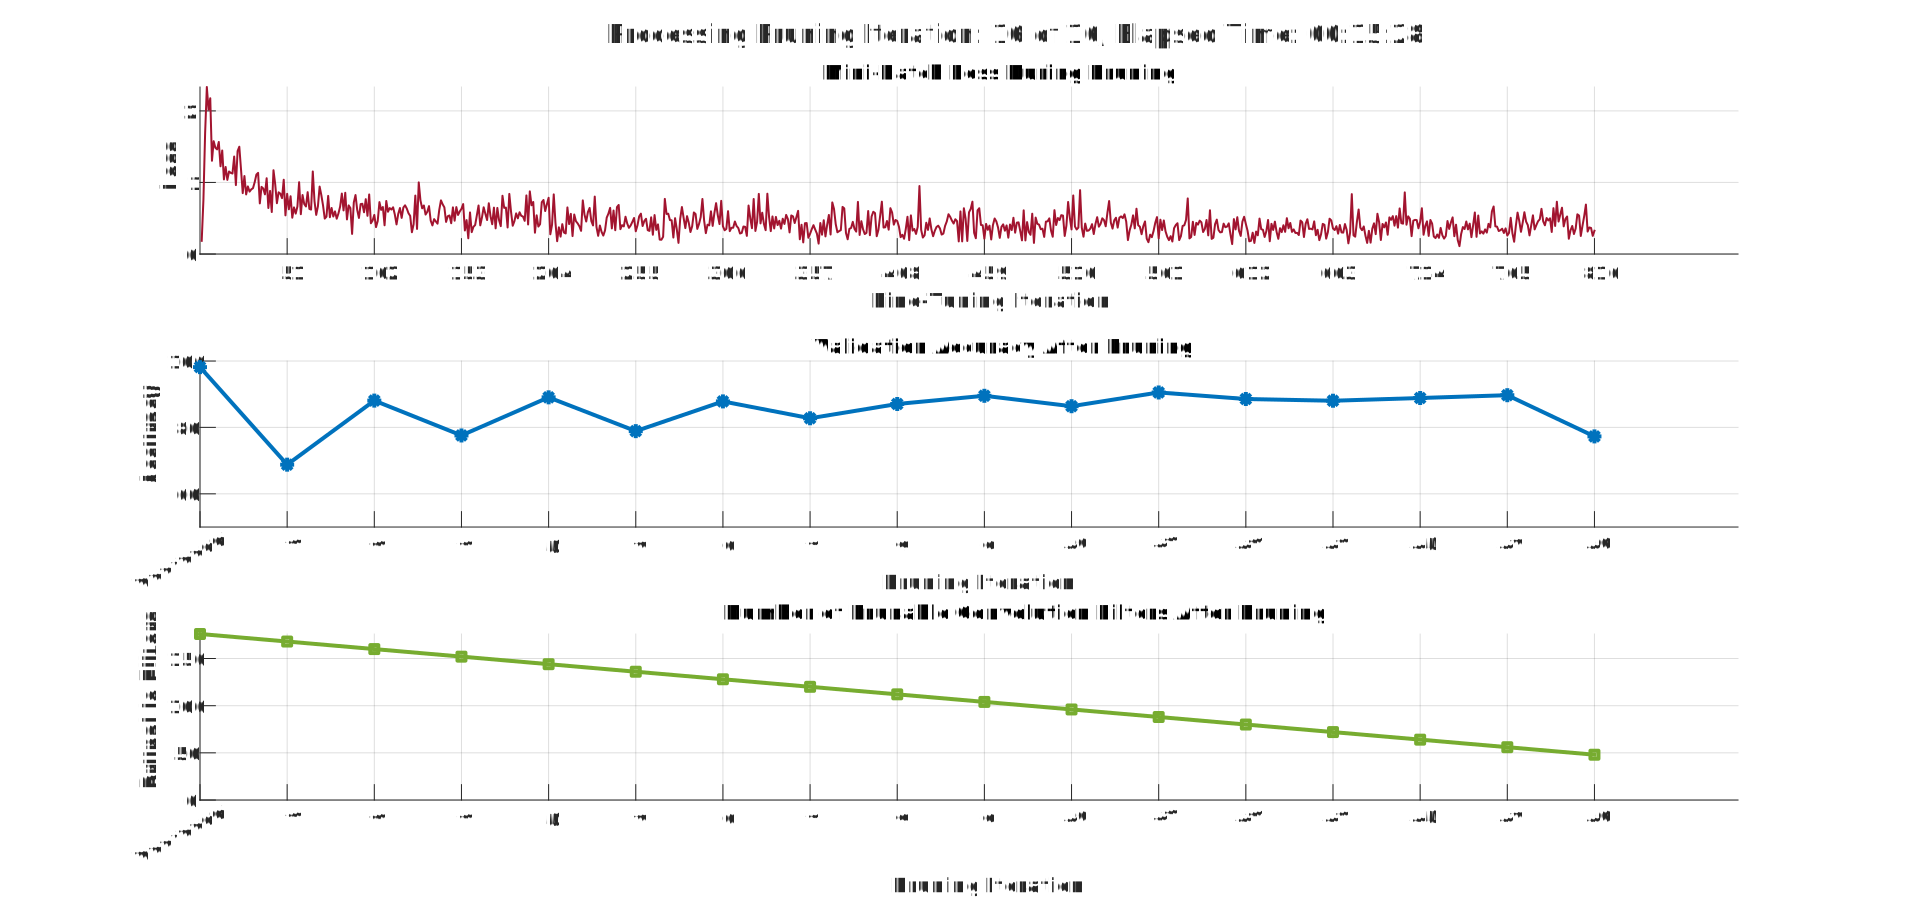
\includegraphics[width=1.0\textwidth]{pruning.png}}
     \end{center} % adjust width as needed
    \caption{Training Progress on a GPU}
    \label{fig:training}
\end{figure}
\textbf{Retraining After Pruning}

Since pruning may lead to a reduction in validation accuracy due to changes in the network structure, the network is retrained after pruning to regain any lost accuracy. The pruned network is reassembled, and the classification layer from the original network is attached.

\begin{center}
\begin{tcolorbox}[breakable, enhanced, boxsep=10pt]
\begin{minted}[fontsize=\footnotesize]{MATLAB}
prunedLayerGraph =  reassembleTaylorNetwork(prunableNet, classes);
\end{minted}
\end{tcolorbox}
\end{center}

Training options are specified, and the network is trained again using the reassembled pruned network.

\begin{center}
\begin{tcolorbox}[breakable, enhanced, boxsep=10pt]
\begin{minted}[fontsize=\footnotesize]{MATLAB}
miniBatchSize = 128;
validationFrequency = floor(numel(TTrain)/miniBatchSize);
options = trainingOptions("sgdm", ...
    InitialLearnRate=3e-4, ...
    MaxEpochs=15, ...
    MiniBatchSize=miniBatchSize, ...
    Shuffle="every-epoch", ...
    Verbose=false, ...
    ValidationData={XValidation,TValidation}, ...
    OutputNetwork="best-validation-loss");
trainedNetPruned = trainNetwork(XTrain,TTrain,prunedLayerGraph,options);
\end{minted}
\end{tcolorbox}
\end{center}
The following is the training progress of the pruned network:
\begin{figure}[H]
    \setlength{\fboxsep}{0pt} % remove spacing inside the box
    \setlength{\fboxrule}{1pt} % adjust border thickness
    \begin{center}
     \fbox{\includegraphics[width=1.0\textwidth]{pruned.png}}
     \end{center} % adjust width as needed
    \caption{Retraining Progress After Pruning}
    \label{fig:training}
\end{figure}
\subsection{Quantization Process}
First, we create a `dlquantizer` object from the pruned network and specify the `ExecutionEnvironment` property as 'GPU':

\begin{center}
\begin{tcolorbox}[breakable, enhanced, boxsep=10pt]
\begin{minted}[linenos, breaklines=true, breakbefore=., fontsize=\footnotesize]
{MATLAB}
dlquantObj = dlquantizer(trainedNetPruned, ExecutionEnvironment='GPU');
\end{minted}
\end{tcolorbox}
\end{center}

Next, we collect calibration statistics using the supporting function `createCalibrationSet` to create a representative calibration datastore with elements from each label in the training data:

\begin{center}
\begin{tcolorbox}[breakable, enhanced, boxsep=10pt]
\begin{minted}[linenos, breaklines=true, breakbefore=., fontsize=\footnotesize]
{MATLAB}
calData = createCalibrationSet(XTrain, TTrain, 36
["yes","no","up","down","left","right","on","off",
"stop","go","unknown","background"]);
calibrate(dlquantObj, calData);
\end{minted}
\end{tcolorbox}
\end{center}

Finally, we quantize the network using the `quantize` function and save the quantized network to a file. We also retrieve and display the quantization details:

\begin{center}
\begin{tcolorbox}[breakable, enhanced, boxsep=10pt]
\begin{minted}[linenos, breaklines=true, breakbefore=., fontsize=\footnotesize]
{MATLAB}
qnetPruned = quantize(dlquantObj, 'ExponentScheme', 'Histogram');
save("qnet", "qnetPruned");
\end{minted}
\end{tcolorbox}
\end{center}

\subsection{Compression Evaluation}
We use the `estimateNetworkMetrics` function to generate network metrics for the original network, the pruned network, and the quantized network:

\begin{center}
\begin{tcolorbox}[breakable, enhanced, boxsep=10pt]
\begin{minted}[linenos, breaklines=true, breakbefore=., fontsize=\footnotesize]
{MATLAB}
originalNetMetrics = estimateNetworkMetrics(trainedNet);
taylorNetMetrics = estimateNetworkMetrics(trainedNetPruned);
quantizedNetMetrics = estimateNetworkMetrics(qnetPruned);
\end{minted}
\end{tcolorbox}
\end{center}

We evaluate the impact of each stage of compression on the number of learnables in the network and the parameter memory of the network.


We extract the parameter memory of each network and visualize them in a bar plot. Taylor pruning significantly reduces the parameter memory of the network, and quantization reduces it further. The combination of Taylor pruning and quantization compresses the deep learning network to meet reduced memory requirements while largely maintaining the accuracy of the deep neural network:

\begin{center}
\begin{tcolorbox}[breakable, enhanced, boxsep=10pt]
\begin{minted}[linenos, breaklines=true, breakbefore=., fontsize=\footnotesize]
{MATLAB}
figure;
memory = [sum(originalNetMetrics.("ParameterMemory (MB)"))
               sum(taylorNetMetrics.("ParameterMemory (MB)"))
               sum(quantizedNetMetrics.("ParameterMemory (MB)"))];
  
plotResults(x, memory)
ylabel("Parameter Memory (MB)")
title("Parameter Memory of Network")
\end{minted}
\end{tcolorbox}
\end{center}
\begin{center}
\includesvg[width=0.8\linewidth]{memory.svg}
\captionof{figure}{Memory comparison of the model after pruning \& quantization}
\end{center}
\newpage
\section{Integration onto the ESP32 Module}
The integration of the command processing system onto the ESP32 module involves several steps to ensure efficient and reliable operation. This section details the process of embedding the command recognition and execution logic into the ESP32.

The code implementation is divided into several crucial components. First, \textbf{\texttt{CommandDetector.cpp}}, then, \textbf{\texttt{CommandProcessor.cpp}}, and finally, \textbf{\texttt{main.cpp}}.
\subsection{Firmware}
\subsubsection{\texttt{CommandDetector.cpp}}
\begin{center}
\begin{tcolorbox}[breakable, enhanced, boxsep=10pt]
\begin{minted}[linenos, breaklines=true, breakbefore=., fontsize=\footnotesize]
{C++}
CommandDetector::CommandDetector(I2SSampler *sample_provider, CommandProcessor *command_procesor)
{
    m_last_detection = 0;
    m_scores_index = 0;
    m_command_processor = command_procesor;
    m_sample_provider = sample_provider;
    m_average_detect_time = 0;
    m_number_of_runs = 0;
    m_nn = new NeuralNetwork();
    Serial.println("Created Neural Net");
    m_audio_processor = new AudioProcessor(AUDIO_LENGTH, WINDOW_SIZE, STEP_SIZE, POOLING_SIZE);
    for (int i = 0; i < COMMAND_WINDOW; i++)
    {
        for (int j = 0; j < NUMBER_COMMANDS; j++)
        {
            m_scores[i][j] = 0;
        }
    }
    m_scores_index = 0;
    Serial.println("Created audio processor");
}
\end{minted}
\end{tcolorbox}
\end{center}

The constructor of the `CommandDetector` class initializes various components required for command detection. It sets up the neural network and audio processor, initializes the command score buffer, and saves references to the sample provider and command processor. Additionally, it initializes performance statistics variables to track detection efficiency.

\begin{center}
\begin{tcolorbox}[breakable, enhanced, boxsep=10pt]
\begin{minted}[linenos, breaklines=true, breakbefore=., fontsize=\footnotesize]
{C++}
CommandDetector::~CommandDetector()
{
    delete m_nn;
    m_nn = NULL;
    delete m_audio_processor;
    m_audio_processor = NULL;
    uint32_t free_ram = esp_get_free_heap_size();
    Serial.printf("Free ram after DetectWakeWord cleanup %d\n", free_ram);
}
\end{minted}
\end{tcolorbox}
\end{center}

The destructor of the `CommandDetector` class ensures that dynamically allocated resources, such as the neural network and audio processor, are properly deallocated. This prevents memory leaks and ensures that the system remains stable and efficient. The destructor also logs the available free memory after cleanup.

\begin{center}
\begin{tcolorbox}[breakable, enhanced, boxsep=10pt]
\begin{minted}[linenos, breaklines=true, breakbefore=., fontsize=\footnotesize]
{C++}
void CommandDetector::run()
{
    long start = millis();
    RingBufferAccessor *reader = m_sample_provider->getRingBufferReader();
    reader->rewind(16000);
    float *input_buffer = m_nn->getInputBuffer();
    bool is_valid = m_audio_processor->get_spectrogram(reader, input_buffer);
    delete reader;
    m_nn->predict();
    for (int i = 0; i < NUMBER_COMMANDS; i++)
    {
        float prediction = std::max(m_nn->getOutputBuffer()[i], 1e-6f);
        m_scores[m_scores_index][i] = log(is_valid ? prediction : 1e-6);
    }
    m_scores_index = (m_scores_index + 1) % COMMAND_WINDOW;
    float scores[NUMBER_COMMANDS] = {0, 0, 0, 0, 0};
    for (int i = 0; i < COMMAND_WINDOW; i++)
    {
        for (int j = 0; j < NUMBER_COMMANDS; j++)
        {
            scores[j] += m_scores[i][j];
        }
    }
    float best_score = scores[0];
    int best_index = 0;
    for (int i = 1; i < NUMBER_COMMANDS; i++)
    {
        if (scores[i] > best_score)
        {
            best_index = i;
            best_score = scores[i];
        }
    }
    long end = millis();
    if (best_score > DETECTION_THRESHOLD && best_index != NUMBER_COMMANDS - 1 && start - m_last_detection > 1000)
    {
        m_last_detection = start;
        m_command_processor->queueCommand(best_index, best_score);
    }
    m_average_detect_time = (end - start) * 0.1 + m_average_detect_time * 0.9;
    m_number_of_runs++;
    if (m_number_of_runs == 100)
    {
        m_number_of_runs = 0;
        Serial.printf("Average detection time %.fms\n", m_average_detect_time);
    }
}
\end{minted}
\end{tcolorbox}
\end{center}

The `run` method is the core of the command detection functionality. It begins by timing the operation for performance statistics. The method retrieves audio samples from a ring buffer, rewinds by one second, and processes the samples into a spectrogram suitable for neural network input. After obtaining predictions from the neural network, it logs the predictions in a sliding window buffer to smooth out detections. The method then aggregates scores to find the best command prediction. If the best score exceeds the detection threshold and the cooldown period has passed, the command is queued for execution. The method also updates performance statistics and logs detection times periodically.

\subsubsection{\texttt{CommandProcessor.cpp}}
\begin{center}
\begin{tcolorbox}[breakable, enhanced, boxsep=10pt]
\begin{minted}[linenos, breaklines=true, breakbefore=., fontsize=\footnotesize]
{C++}
#include <Arduino.h>
#include "CommandProcessor.h"

const char *words[] = {
    "forward",
    "backward",
    "left",
    "right",
    "_nonsense",
};
\end{minted}
\end{tcolorbox}
\end{center}

This snippet includes the necessary libraries, specifically `Arduino.h` for standard Arduino functions and a custom header file `CommandProcessor.h` which contains the definition of the `CommandProcessor` class.

\begin{center}
\begin{tcolorbox}[breakable, enhanced, boxsep=10pt]
\begin{minted}[linenos, breaklines=true, breakbefore=., fontsize=\footnotesize]
{C++}
void commandQueueProcessorTask(void *param)
{
    CommandProcessor *commandProcessor = (CommandProcessor *)param;
    while (true)
    {
        uint16_t commandIndex = 0;
        if (xQueueReceive(commandProcessor->m_command_queue_handle, &commandIndex, portMAX_DELAY) == pdTRUE)
        {
            commandProcessor->processCommand(commandIndex);
        }
    }
}
\end{minted}
\end{tcolorbox}
\end{center}

This function defines a task that runs indefinitely, waiting for commands from a queue. The `commandQueueProcessorTask` function continuously checks the queue for new commands using `xQueueReceive`. When a command is received, it is processed by calling the `processCommand` method of the `CommandProcessor` class. The `param` parameter is cast to a `CommandProcessor` pointer, allowing access to the class methods and attributes.


\begin{center}
\begin{tcolorbox}[breakable, enhanced, boxsep=10pt]
\begin{minted}[linenos, breaklines=true, breakbefore=., fontsize=\footnotesize]
{C++}
int calcDuty(int ms)
{
    // 50Hz = 20ms period
    return (65536 * ms) / 20000;
}
\end{minted}
\end{tcolorbox}
\end{center}

The `calcDuty` function calculates the duty cycle for a 50Hz Pulse Width Modulation (PWM) signal based on the input duration in milliseconds. Given that a 50Hz signal has a period of 20ms, the function computes the duty cycle by scaling the input duration to the PWM resolution, which is typically 16 bits (65536 levels). The return value is used to set the PWM signal for control.



\begin{center}
\begin{tcolorbox}[breakable, enhanced, boxsep=10pt]
\begin{minted}[linenos, breaklines=true, breakbefore=., fontsize=\footnotesize]
{C++}
CommandProcessor::CommandProcessor()
{
    pinMode(GPIO_NUM_2, OUTPUT);
    // setup the motors
    ledcSetup(0, 50, 16);
    ledcAttachPin(GPIO_NUM_13, 0);
    ledcSetup(1, 50, 16);
    ledcAttachPin(GPIO_NUM_12, 1);
    ledcWrite(0, calcDuty(1500)); // left
    ledcWrite(1, calcDuty(1500)); // right

    // allow up to 5 commands to be in flight at once
    m_command_queue_handle = xQueueCreate(5, sizeof(uint16_t));
    if (!m_command_queue_handle)
    {
        Serial.println("Failed to create command queue");
    }
    // kick off the command processor task
    TaskHandle_t command_queue_task_handle;
    xTaskCreate(commandQueueProcessorTask, "Command Queue Processor", 1024, this, 1, &command_queue_task_handle);
}
\end{minted}
\end{tcolorbox}
\end{center}

The constructor for the `CommandProcessor` class initializes the necessary hardware and sets up the command processing infrastructure. It sets the GPIO pin mode for an output pin, sets up two PWM channels for control, and initializes them with a neutral (stop) duty cycle. The constructor also creates a queue to hold commands, with a capacity for up to five commands. If queue creation fails, it prints an error message. Finally, it starts the command processing task, `commandQueueProcessorTask`, which runs independently to process commands from the queue.

\begin{center}
\begin{tcolorbox}[breakable, enhanced, boxsep=10pt]
\begin{minted}[linenos, breaklines=true, breakbefore=., fontsize=\footnotesize]
{C++}
void CommandProcessor::queueCommand(uint16_t commandIndex, float best_score)
{
    if (commandIndex != 5 && commandIndex != -1)
    {
        Serial.printf("***** %ld Detected command %s(%f)\n", millis(), words[commandIndex], best_score);
        if (xQueueSendToBack(m_command_queue_handle, &commandIndex, 0) != pdTRUE)
        {
            Serial.println("No more space for command");
        }
    }
}
\end{minted}
\end{tcolorbox}
\end{center}

The `queueCommand` method queues a command to be processed, provided it is valid (not equal to 5 or -1). It prints a message to the serial monitor indicating the detected command and its confidence score. If the queue is full, it prints an error message indicating that there is no more space for the command. This method ensures that valid commands are enqueued for processing, allowing the system to handle multiple commands in sequence.

\subsubsection{\texttt{main.cpp}}
The main application for command detection on the ESP32 module orchestrates the setup and operation of the entire system. This section details the implementation of the main application, including the configuration of I2S (Inter-IC Sound) for audio input, the creation of tasks for processing commands, and the initialization and running of the main loop.

\begin{center}
\begin{tcolorbox}[breakable, enhanced, boxsep=10pt]
\begin{minted}[linenos, breaklines=true, breakbefore=., fontsize=\footnotesize]
{C++}
#include <Arduino.h>
#include <WiFi.h>
#include <driver/i2s.h>
#include <esp_task_wdt.h>
#include "I2SMicSampler.h"
#include "ADCSampler.h"
#include "config.h"
#include "CommandDetector.h"
#include "CommandProcessor.h"
\end{minted}
\end{tcolorbox}
\end{center}

This snippet includes the necessary libraries for Arduino functionalities, WiFi, I2S audio interface, and the watchdog timer. Additionally, it includes headers for custom classes handling microphone sampling, command detection, and processing.

\begin{center}
\begin{tcolorbox}[breakable, enhanced, boxsep=10pt]
\begin{minted}[linenos, breaklines=true, breakbefore=., fontsize=\footnotesize]
{C++}
i2s_config_t adcI2SConfig = {
    .mode = (i2s_mode_t)(I2S_MODE_MASTER | I2S_MODE_RX | I2S_MODE_ADC_BUILT_IN),
    .sample_rate = 16000,
    .bits_per_sample = I2S_BITS_PER_SAMPLE_16BIT,
    .channel_format = I2S_CHANNEL_FMT_ONLY_LEFT,
    .communication_format = I2S_COMM_FORMAT_I2S_LSB,
    .intr_alloc_flags = ESP_INTR_FLAG_LEVEL1,
    .dma_buf_count = 4,
    .dma_buf_len = 64,
    .use_apll = false,
    .tx_desc_auto_clear = false,
    .fixed_mclk = 0};
\end{minted}
\end{tcolorbox}
\end{center}

\begin{center}
\begin{tcolorbox}[breakable, enhanced, boxsep=10pt]
\begin{minted}[linenos, breaklines=true, breakbefore=., fontsize=\footnotesize]
{C++}
i2s_config_t i2sMemsConfigBothChannels = {
    .mode = (i2s_mode_t)(I2S_MODE_MASTER | I2S_MODE_RX),
    .sample_rate = 16000,
    .bits_per_sample = I2S_BITS_PER_SAMPLE_32BIT,
    .channel_format = I2S_MIC_CHANNEL,
    .communication_format = i2s_comm_format_t(I2S_COMM_FORMAT_I2S),
    .intr_alloc_flags = ESP_INTR_FLAG_LEVEL1,
    .dma_buf_count = 4,
    .dma_buf_len = 64,
    .use_apll = false,
    .tx_desc_auto_clear = false,
    .fixed_mclk = 0};
\end{minted}
\end{tcolorbox}
\end{center}

These snippets define the I2S configurations for two different setups: using the internal ADC and reading from both channels of an I2S microphone. Each configuration specifies the mode, sample rate, bit depth, channel format, communication format, and other parameters necessary for the proper operation of the I2S interface.

\begin{center}
\begin{tcolorbox}[breakable, enhanced, boxsep=10pt]
\begin{minted}[linenos, breaklines=true, breakbefore=., fontsize=\footnotesize]
{C++}
i2s_pin_config_t i2s_mic_pins = {
    .bck_io_num = I2S_MIC_SERIAL_CLOCK,
    .ws_io_num = I2S_MIC_LEFT_RIGHT_CLOCK,
    .data_out_num = I2S_PIN_NO_CHANGE,
    .data_in_num = I2S_MIC_SERIAL_DATA};
\end{minted}
\end{tcolorbox}
\end{center}

This snippet sets the I2S pin configuration for the microphone, specifying the pin numbers for the serial clock, left-right clock, and serial data input.

\begin{center}
\begin{tcolorbox}[breakable, enhanced, boxsep=10pt]
\begin{minted}[linenos, breaklines=true, breakbefore=., fontsize=\footnotesize]
{C++}
void applicationTask(void *param)
{
  CommandDetector *commandDetector = static_cast<CommandDetector *>(param);

  const TickType_t xMaxBlockTime = pdMS_TO_TICKS(100);
  while (true)
  {
    uint32_t ulNotificationValue = ulTaskNotifyTake(pdTRUE, xMaxBlockTime);
    if (ulNotificationValue > 0)
    {
      commandDetector->run();
    }
  }
}
\end{minted}
\end{tcolorbox}
\end{center}

The `applicationTask` function is the main task that handles the heavy lifting of the application. It runs in an infinite loop, waiting for notifications that audio samples are available. When notified, it calls the `run` method of the `CommandDetector` to process the audio samples and detect commands.

\begin{center}
\begin{tcolorbox}[breakable, enhanced, boxsep=10pt]
\begin{minted}[linenos, breaklines=true, breakbefore=., fontsize=\footnotesize]
{C++}
void setup()
{
  Serial.begin(115200);
  delay(1000);
  Serial.println("Starting up");

  esp_task_wdt_init(10, false);

#ifdef USE_I2S_MIC_INPUT
  I2SSampler *i2s_sampler = new I2SMicSampler(i2s_mic_pins, false);
#else
  I2SSampler *i2s_sampler = new ADCSampler(ADC_UNIT_1, ADC_MIC_CHANNEL);
#endif

  CommandProcessor *command_processor = new CommandProcessor();

  CommandDetector *commandDetector = new CommandDetector(i2s_sampler, command_processor);

  TaskHandle_t applicationTaskHandle;
  xTaskCreatePinnedToCore(applicationTask, "Command Detect", 8192, commandDetector, 1, &applicationTaskHandle, 0);

}
\end{minted}
\end{tcolorbox}
\end{center}

The `setup` function initializes the serial communication, sets up the watchdog timer to prevent task killing, and configures the I2S input depending on the type of microphone used (I2S or ADC). It creates instances of `I2SSampler`, `CommandProcessor`, and `CommandDetector` classes. It also creates and pins the application task to a specific core. Finally, it starts sampling from the I2S device using the appropriate configuration.

\begin{center}
\begin{tcolorbox}[breakable, enhanced, boxsep=10pt]
\begin{minted}[linenos, breaklines=true, breakbefore=., fontsize=\footnotesize]
{C++}
void loop()
{
  vTaskDelay(pdMS_TO_TICKS(1000));
}
\end{minted}
\end{tcolorbox}
\end{center}

The `loop` function runs indefinitely with a delay of one second. This is a placeholder loop as the main work is done in the `applicationTask`.

\chapter*{General Conclusion}
\addcontentsline{toc}{chapter}{General Conclusion}
In conclusion, this project has successfully explored the feasibility of an end-to-end voice command security system leveraging deep learning on microcontrollers. The core of the system, a convolutional neural network (CNN), demonstrated promising results in recognizing specific voice commands with high accuracy. This paves the way for hands-free, voice-based interaction with critical systems, potentially leading to significant safety and efficiency gains, particularly in real-world scenarios with high complexity or hazardous environments.
\\
However, further advancements are necessary to address certain limitations. Speech recognition robustness remains a key area for improvement. The model's ability to accurately recognize commands amidst background noise and speaker variations needs rigorous evaluation. Additionally, deploying this system on resource-constrained microcontrollers necessitates addressing computational efficiency. Finding an optimal balance between accuracy and computational cost will be crucial for real-world implementation.
\\
Future research efforts should explore several avenues. Integrating the system with existing security protocols will ensure seamless compatibility and enhance overall security posture. Additionally, incorporating speaker identification capabilities could offer an additional security layer. Furthermore, investigating transfer learning techniques for CNNs could potentially improve recognition accuracy while reducing training data requirements, making the system more adaptable to diverse environments.
\\
In essence, this project has made significant strides in the development of AI-powered security systems using speech recognition and deep learning on microcontrollers. By addressing the identified limitations and pursuing the proposed future research directions, this approach has the potential to revolutionize security practices across various domains.
\begin{thebibliography}{10}
\pagenumbering{roman}
\setcounter{page}{7} 
\addcontentsline{toc}{chapter}{Webliography}

\bibitem{dataset}
Warden P. "Speech Commands: A public dataset for single-word speech recognition", Google Copyright 2017. Available from\\
\url{http://download.tensorflow.org/data/speech_commands_v0.01.tar.gz}

\bibitem{matlab}
    Train Speech Command Recognition Model Using Deep Learning,\\
\url{https://www.mathworks.com/help/deeplearning/ug/deep-learning-speech-recognition.html}

\bibitem{tensorflow}
    Introduction to graphs and tf.function,\\
    \url{https://www.tensorflow.org/guide/intro_to_graphs#:~:text=TensorFlow\%20uses\%20graphs\%20as\%20the,(\%22constant\%20folding\%22).}
\bibitem{CNN_speech_recognition}
    Convolutional Neural Networks for Speech Recognition (2014),\\
    \url{https://www.microsoft.com/en-us/research/wp-content/uploads/2016/02/CNN_ASLPTrans2-14.pdf}

\bibitem{prune}
    Prune and Quantize Convolutional Neural Network for Speech Recognition,\\
\url{https://www.mathworks.com/help/deeplearning/ug/prune-and-quantize-convolutional-neural-network-for-speech-recognition.html}

\bibitem{lstm}
    Long Short-Term Memory Recurrent Neural Network for Automatic Speech Recognition,\\
    \url{https://www.researchgate.net/publication/359410664_Long_Short-Term_Memory_Recurrent_Neural_Network_for_Automatic_Speech_Recognition}
    
\bibitem{TinyML}
    Retrain a speech recognition model with TensorFlow Lite Model Maker,\\
\url{https://www.tensorflow.org/lite/models/modify/model_maker/speech_recognition?fbclid=IwAR3S8ahImF5ZHanItmlpGbf2JnlShir-\\4wIvCOecd4nVNcYdzl99i-JOkVE}

\bibitem{microsoft}
    THE MICROSOFT 2017 CONVERSATIONAL SPEECH RECOGNITION SYSTEM,\\
    \url{https://www.microsoft.com/en-us/research/wp-content/uploads/2017/08/ms_swbd17-2.pdf}
\bibitem{ibm}
    What is speech recognition?,\\
\url{https://www.ibm.com/topics/speech-recognition}

\bibitem{IEEE_security_privacy}
    STATE-OF-THE-ART SPEECH RECOGNITION WITH SEQUENCE-TO-SEQUENCE MODELS,\\
    \url{https://static.googleusercontent.com/media/research.google.com/en//pubs/archive/46687.pdf}
    
\bibitem{espressif}
    ESP-IDF Programming Guide,\\
    \url{https://docs.espressif.com/projects/esp-idf/en/stable/esp32/index.html}
    
\bibitem{openai}
    OpenAI Whisper Model,\\
    \url{https://github.com/openai/whisper}

\bibitem{github}
    Speech recognition using ESP32 \& Wit.ai,\\
    \url{https://github.com/atomic14/diy-alexa}
    
\bibitem{math}
    Mathematical Theory of Neural Network Models,\\
    \url{https://dataspace.princeton.edu/handle/88435/dsp01xp68kk143}
    
\bibitem{math2}
    A Mathematical Introduction to Neural Networks,\\
    \url{https://diposit.ub.edu/dspace/bitstream/2445/180441/2/tfm_lichtner_bajjaoui_aisha.pdf}
    
\bibitem{IEEXplore}
    Robust Speech Emotion Recognition Using
CNN+LSTM Based on Stochastic Fractal
Search Optimization Algorithm,\\
    \url{https://ieeexplore.ieee.org/document/9770097/}

\bibitem{tflite}
    TensorFlow Lite,\\
    \url{https://www.tensorflow.org/lite/guide}

\bibitem{TikZ}
    Convolutional Neural Network Visualization,\\
    \url{https://tikz.net/neural_networks/}
   
    
\end{thebibliography}
\newpage
\clearpage
\thispagestyle{plain}
\begin{center}
    \vspace*{\fill}
    \includegraphics[width=3cm]{github.png} % Adjust the width as needed
    \vspace{0.5cm} % Adjust vertical space between image and text
    \par % Start a new paragraph for the text
    \textit{The source code for this project is available on GitHub:}\\
    \href{https://github.com/aamar-git/PFE/tree/main}{\texttt{https://github.com/aamar-git/PFE/tree/main}}
    
    \vspace{1cm} % Add additional vertical space
    \copyright{} \textbf{IGEE} 2024 % Add the copyright symbol and the year
    \vspace*{\fill}
\end{center}
\doclicenseThis
\end{document}